\chapter{Search for MSSM $\PH \to hh \to \Pgt\Pgt bb$}
\label{chap:Hhh}
\cite{}
As described in detail in section~\ref{sec:mssmscenarios}, there are many popular
\ac{MSSM} models which can incorporate a $125~\GeV$ Higgs consistent with the boson
discovered at the LHC. As seen in chapter \ref{chap:htt-mssm}, the 
$\Pphi \to \Pgt\Pgt$ analysis is very successful in 
setting limits on various \ac{MSSM} models. The $\Pphi \to \Pgt \Pgt$ result primarily sets
limits on the high $\tan\beta$ regions, and so with large amounts of the
$m_{A}-\tan\beta$ plane ruled out for such \ac{MSSM} scenarios, focus shifts more 
to the regions which are still allowed, in particular at low $\tan\beta$ values.

As discussed in section~\ref{sec:mssmlowtanb}, in certain low $\tan\beta$ regions 
of the \ac{MSSM}, the branching ratio for the
decay of the heavy neutral scalar Higgs, $\PH$, into two of the light Higgs
bosons, $\Ph$, BR($\PH \to \Ph\Ph$), is large. Thus models in which the
light Higgs $\Ph$ has a mass of $125~\GeV$ and is the Higgs particle discovered at the
LHC can be studied via production of a pair of such bosons from a
heavier Higgs $\PH$. As illustrated by figure~\ref{fig:BRlowtanb}, the range of heavy 
Higgs masses of relevance to such a search in the \ac{MSSM} is from $m_{\PH}\approx260~\GeV$ 
(driven by the kinematic threshold for the producton of two $125~\GeV$ Higgs
bosons) up to $m_{\PH}\approx350~\GeV$, above which the branching ratio for 
$\PH$ decaying into tops becomes overwhelmingly high.

In searching for two $125~\GeV$ Higgs bosons, the final state consisting of two
$\tau$ leptons and two $\Pqb$ quarks combines the higher branching ratio of the
$\Ph$ into $\Pqb$ quarks with the relative cleanness of a final state containing
taus. A natural way to search for such a final state is to use the inclusive
selection already defined by the $\PH\to\Pgt\Pgt$ analysis, and require
additional b-jets to form the $\Ph\to\Pqb\Pqb$ part of the final state. 
In this way a large amount of the methods discussed in chapters 
\ref{chap:htt-sm} and \ref{chap:htt-mssm}, 
can be applied to this new analysis targeting $\PH \to \Ph\Ph \to \Pgt\Pgt
\Pqb\Pqb$.

\section{Event Selection and Categorisation}
\label{sec:HhhEventSelection}

The inclusive selection of the di-tau candidate pair is identical to that of
\ac{MSSM} $\Pphi\to\Pgt\Pgt$ analysis discussed in
section~\ref{sec:mssmEventSelection}. On top of the selection of a candidate
$\Pgt\Pgt$ pair, a $\PH \to \Ph\Ph \to \Pgt\Pgt \Pqb\Pqb$ signal would consist of two
$\Pqb$ quarks which hadronise to form b-jets. Thus events used in this analysis
must have a minimum of two jets in order to reconstruct the $\Ph\to\Pqb\Pqb$
part. A selection similar to that
used in the b--tag category of the \ac{MSSM} analysis, in which events are only
selected which contain at least one jet passing the medium \ac{CSV} b-tagging working
point, could be used to select the majority of the $\PH \to \Ph\Ph \to \Pgt\Pgt \Pqb\Pqb$
signal. However, there are a couple of improvements that can be made in
selecting the b-jet candidates for this analysis.

Firstly, the $\pt$ cut on selected jets is lowered from
$30~\GeV$ to $20~\GeV$. The reason for this is that for signal of the type
$\PH\to\Ph\Ph\to\Pgt\Pgt\Pqb\Pqb$, where $m_{\PH}$ is only slightly larger than
$2\times m_{\Ph}$, the final state products will be fairly soft. Thus a higher
$\pt$ cut on the jets will cut out too much signal. 
Figure~\ref{fig:Hhhnjets} indicates the number of jets in inclusive
events in the $\etau$ and $\mutau$ final states, and figure~\ref{fig:Hhhnbjets}
indicates the number of these jets which are b-tagged. Two conclusions can be
drawn from these plots. Firstly, signal events can contain large numbers of
jets. Secondly, the signal does not always contain two jets passing the medium
\ac{CSV} working point; in fact the majority of the events have 0 or 1 b-tagged
jet. The latter indicates that in many events the b-jets in signal resulting
from the true $\Ph\to\Pqb\Pqb$ process are either not inside the jet acceptance
or do not pass the medium \ac{CSV} working point. This means that there is a
high probability that if the jets are ordered for selection according to their
$\pt$ value, the two leading selected jets will not be the correct jets
originating from the $\Pqb$ quarks. A higher success rate for selecting the
correct two jets is achieved if the jets are ordered by their \ac{CSV}
discriminator value, and the two jets with the highest \ac{CSV} discriminator
value are taken to be the $\Ph\to\Pqb\Pqb$ candidate. Figure\ref{fig:Hhhcsv} 
shows the \ac{CSV} values for the leading and subleading
jets in the $\mutau$ channel, when the jets are ordered in this way.

\begin{figure}
\begin{center}
\subfloat[]{
    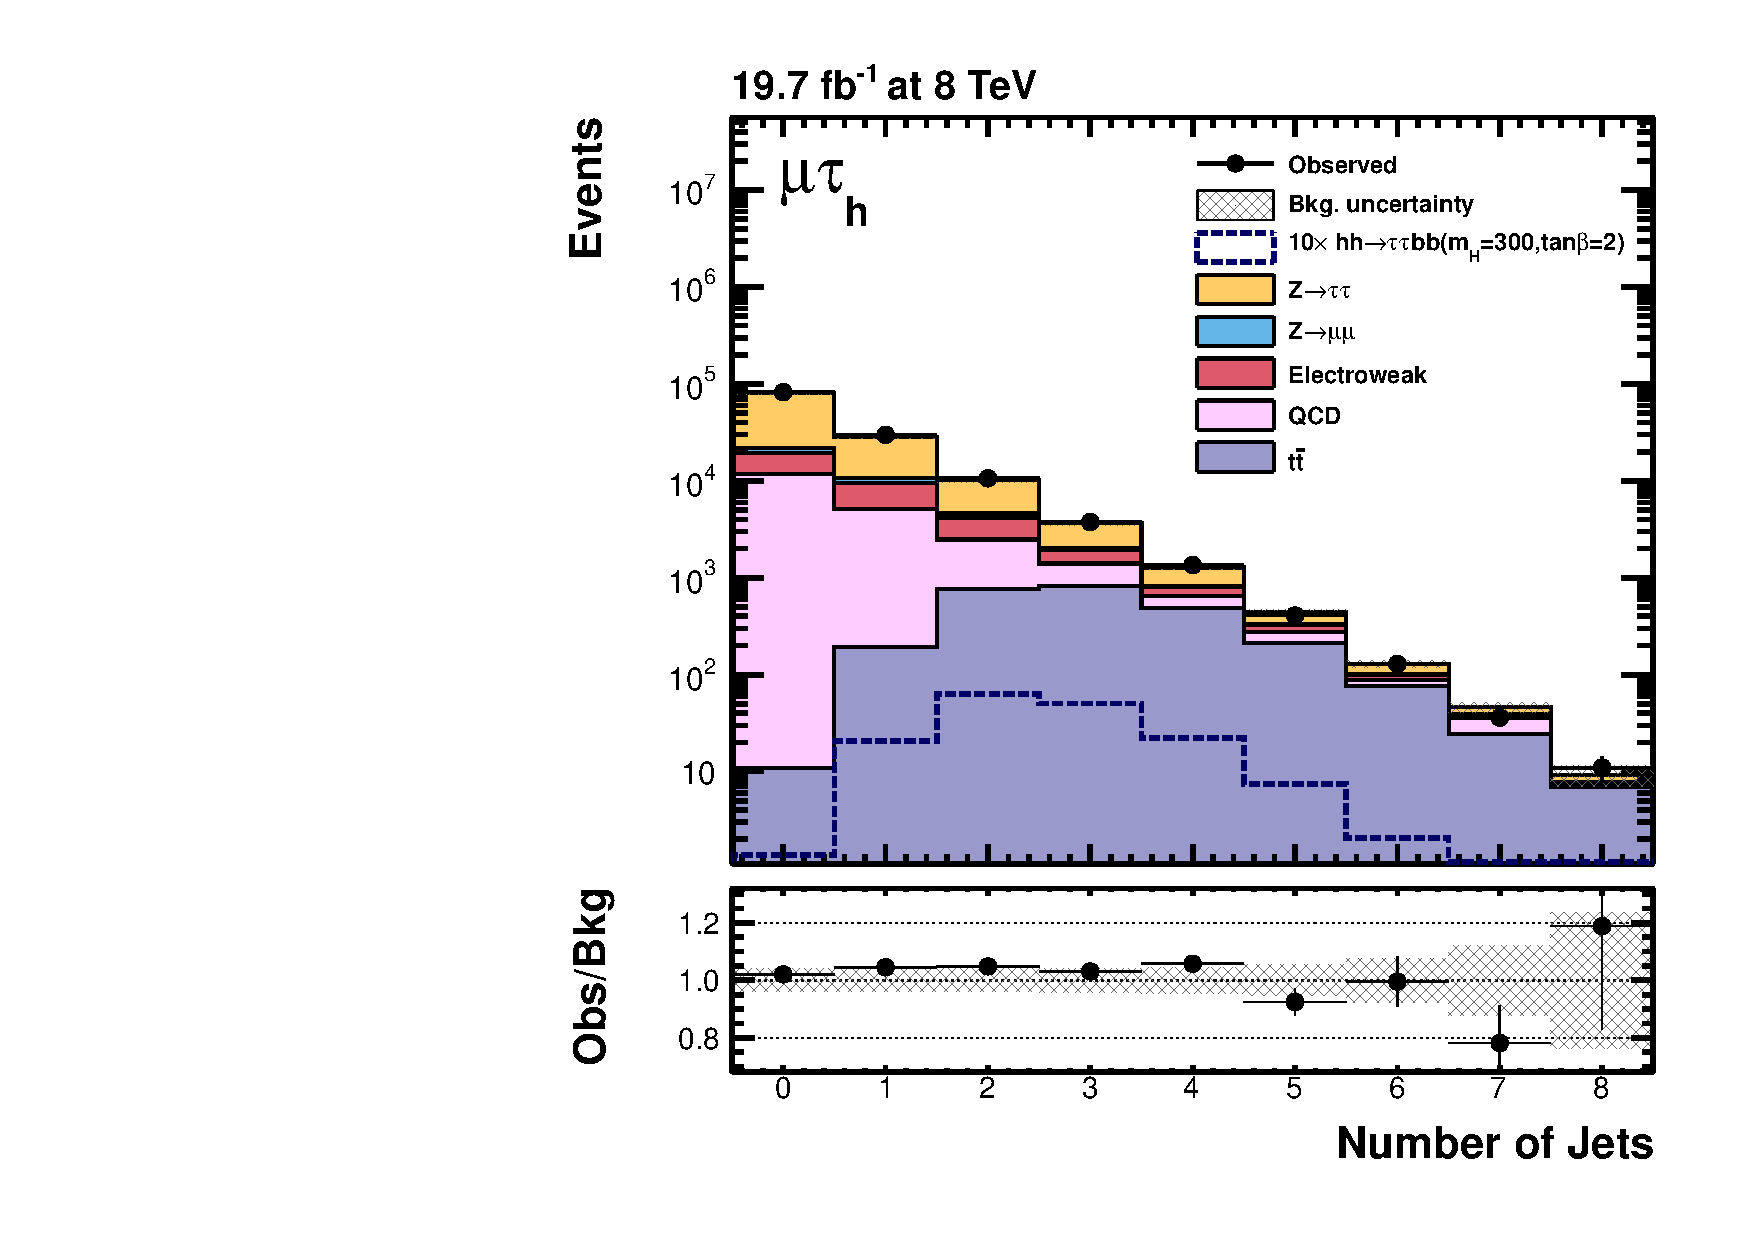
\includegraphics[width=0.5\textwidth]
      {plots/Hhh/n_prebjets_inclusive_mt_2012_log.pdf}}
\subfloat[]{
    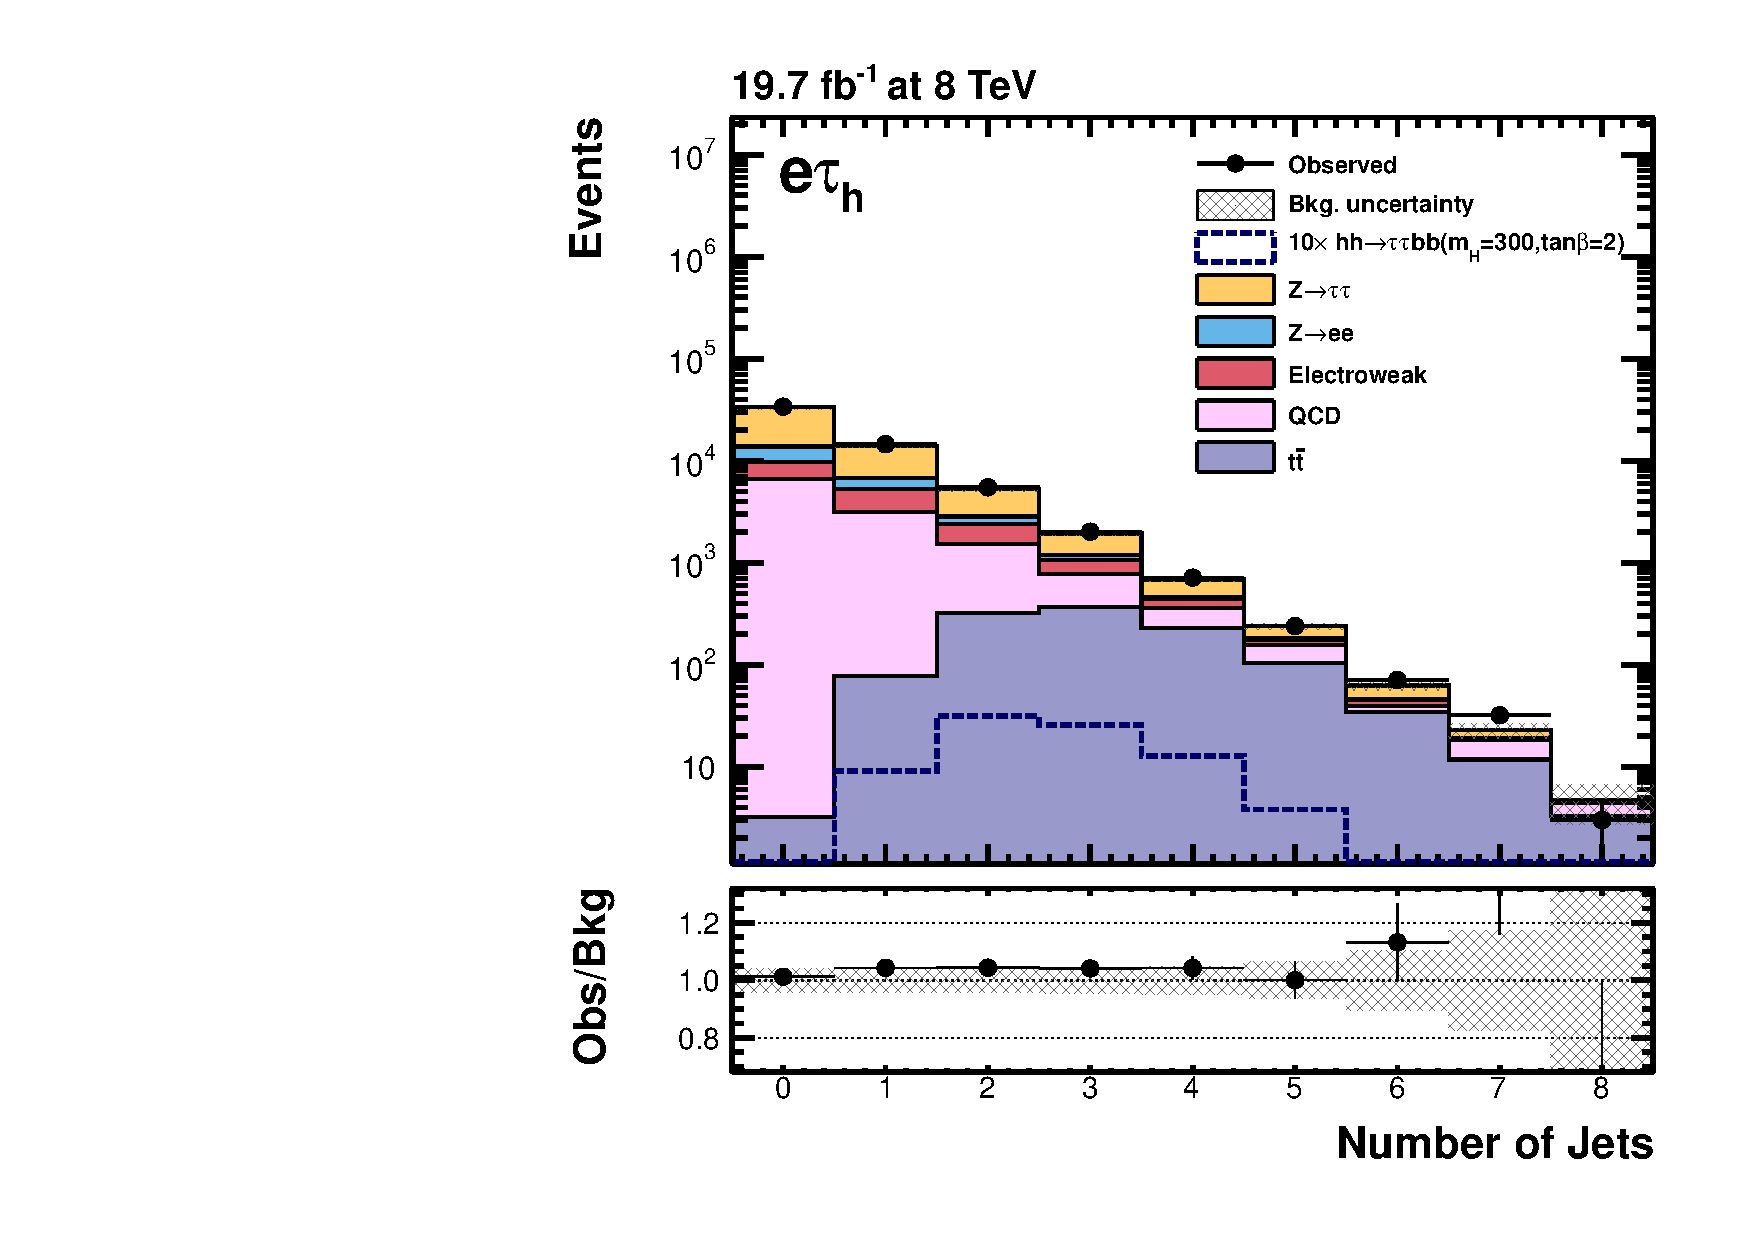
\includegraphics[width=0.5\textwidth] 
      {plots/Hhh/n_prebjets_inclusive_et_2012_log.pdf}} 

\end{center}
\caption{
Number jets in inclusive $\Pgt\Pgt$ events in backgrounds and
$\Ph\to\Ph\Ph$ signal. Distribution shown for the $\mutau$ (left) and $\etau$
(right) channels. }
\label{fig:Hhhbjets}
\end{figure} 

\begin{figure}
\begin{center}
\subfloat[]{
    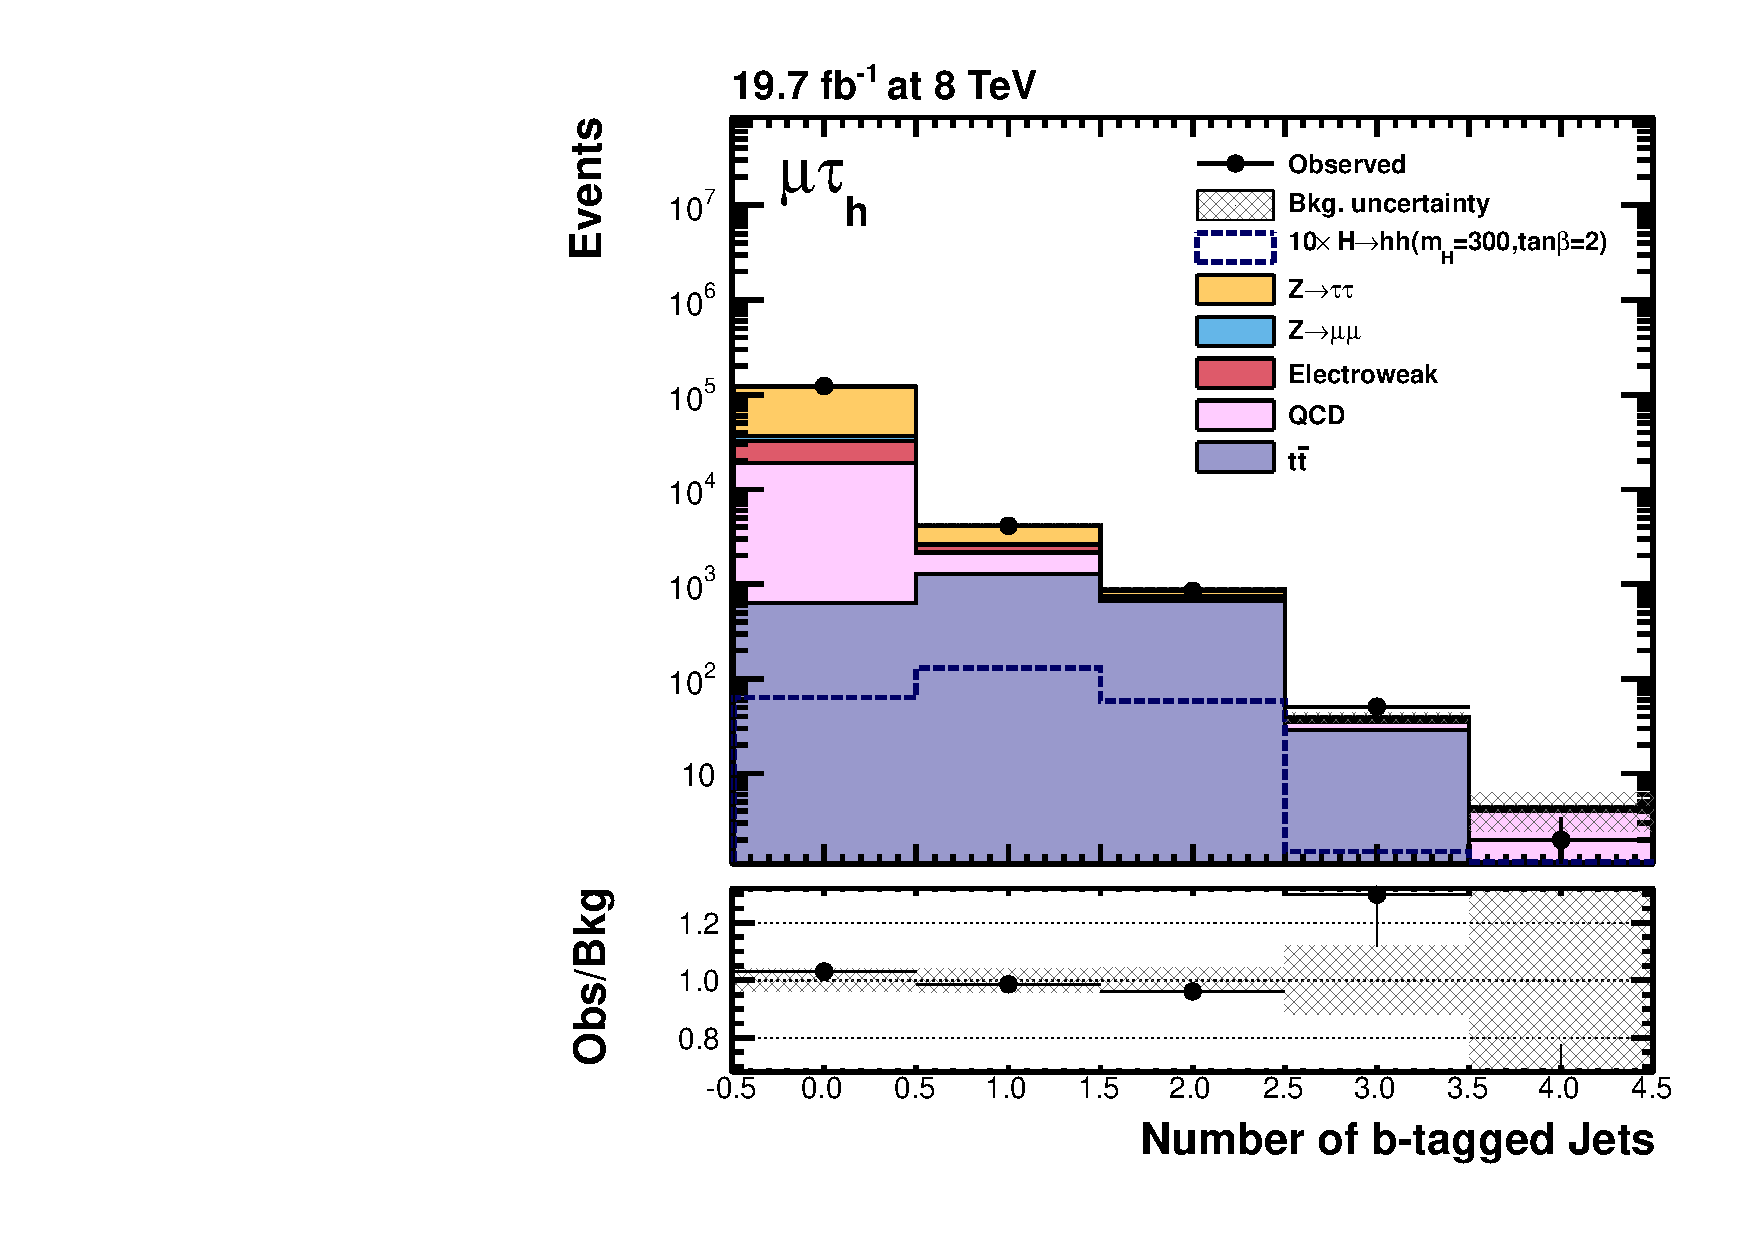
\includegraphics[width=0.5\textwidth]
      {plots/Hhh/n_prebjets_SF_inclusive_mt_2012_log.pdf}}
\subfloat[]{
    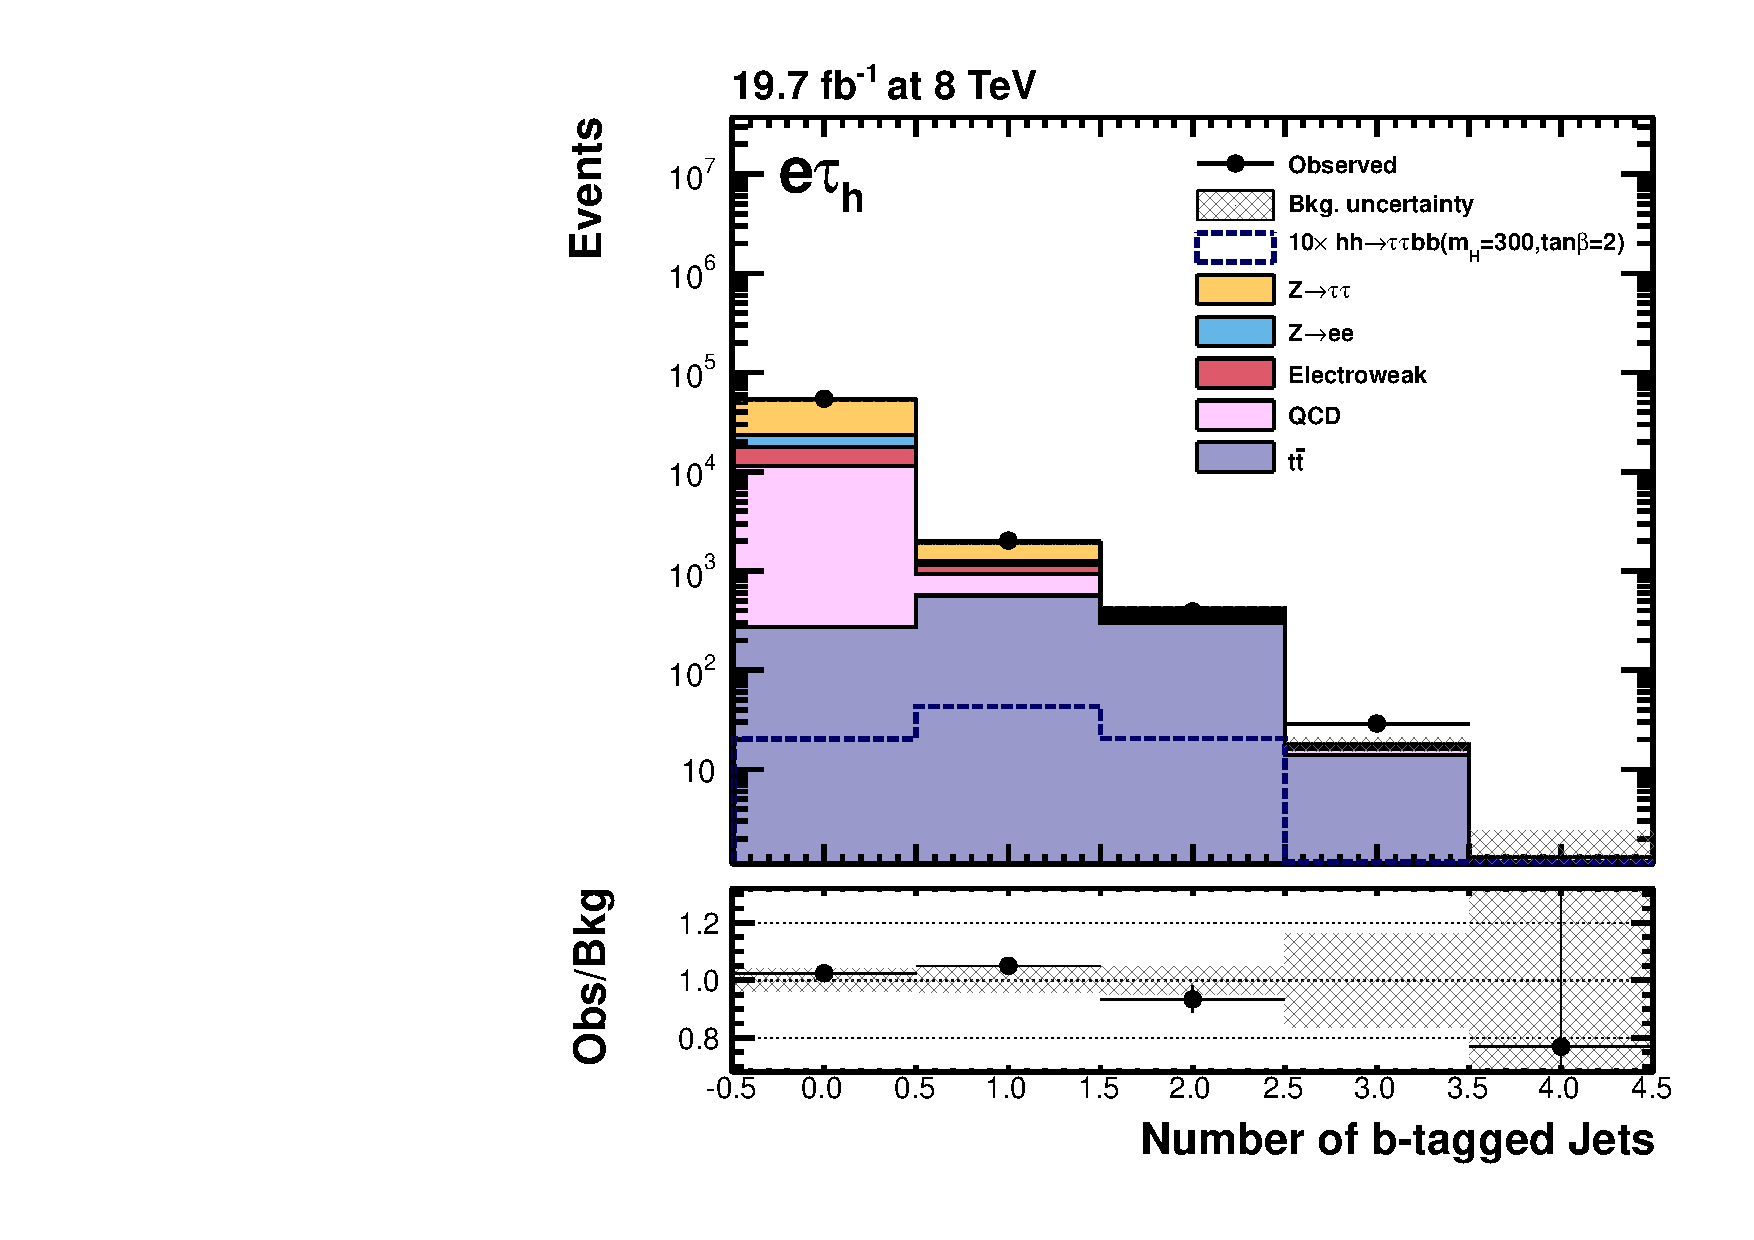
\includegraphics[width=0.5\textwidth] 
      {plots/Hhh/n_prebjets_SF_inclusive_et_2012_log.pdf}} 

\end{center}
\caption{
Number of b-tagged jets in inclusive $\Pgt\Pgt$ events in backgrounds and
$\Ph\to\Ph\Ph$ signal. Distribution shown for the $\mutau$ (left) and $\etau$
(right) channels. }
\label{fig:Hhhnbjets}
\end{figure} 


\begin{figure}
\begin{center}
\subfloat[]{
    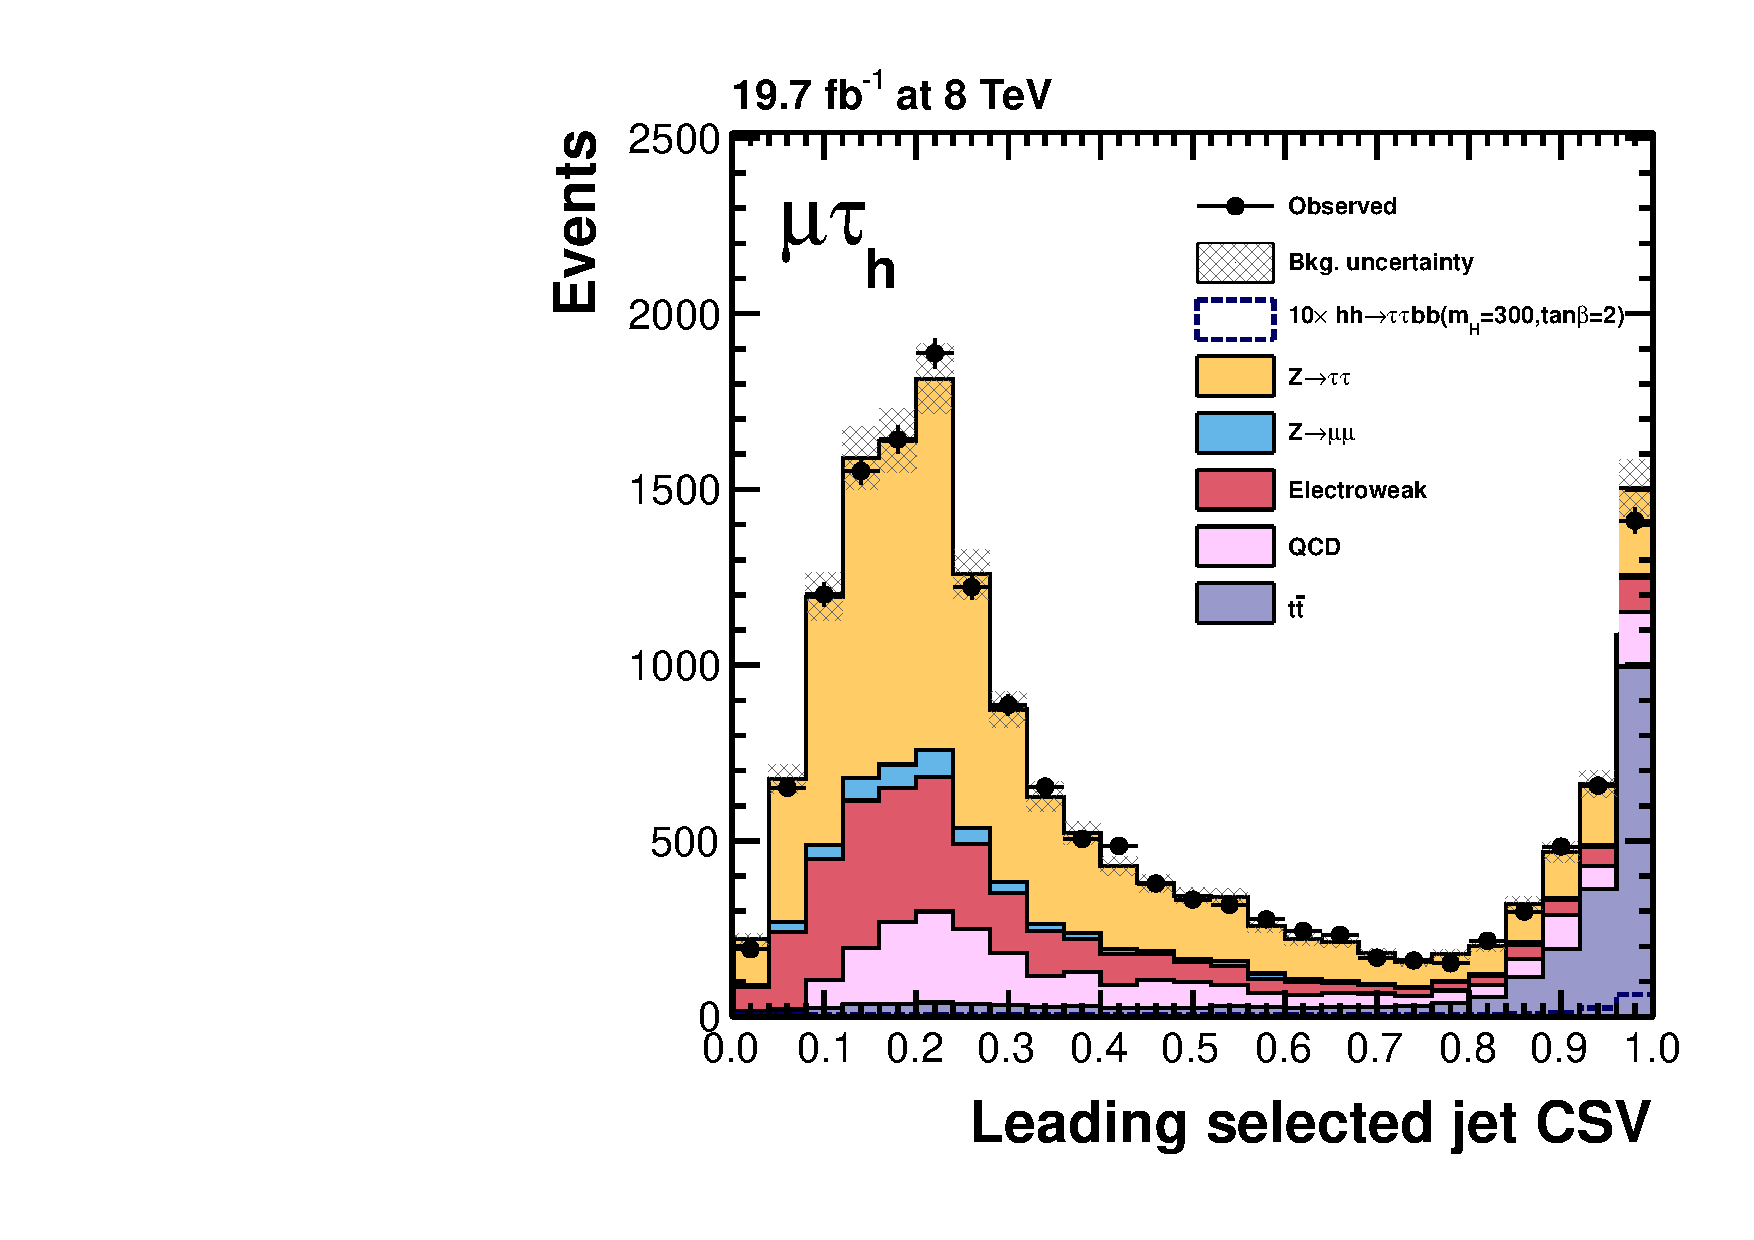
\includegraphics[width=0.5\textwidth]
      {plots/Hhh/prebjetbcsv_1_2jetinclusive_mt_2012.pdf}}
\subfloat[]{
    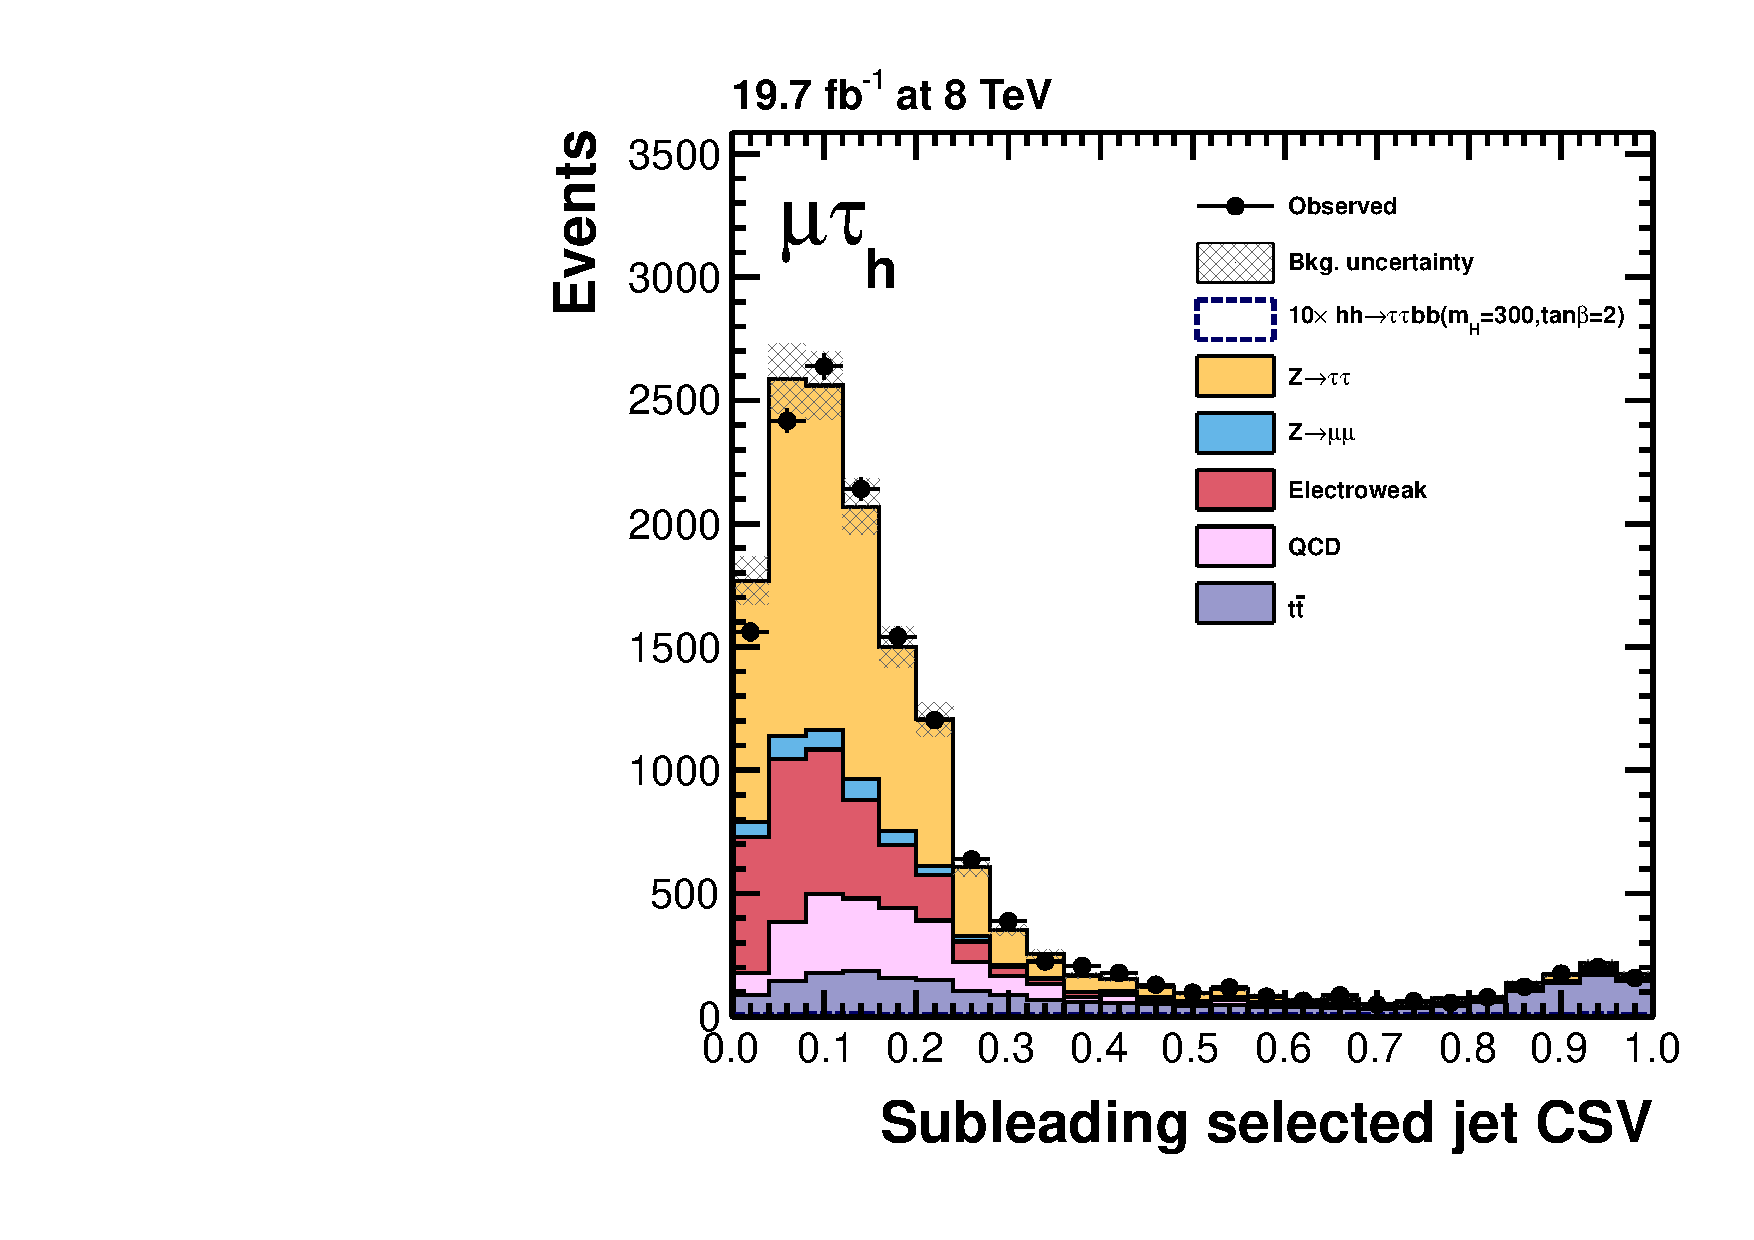
\includegraphics[width=0.5\textwidth] 
      {plots/Hhh/prebjetbcsv_2_2jetinclusive_mt_2012.pdf}} 

\end{center}
\caption{
Values of the \ac{CSV} b-tagging discriminator for the highest \ac{CSV}
(leading) jet in the event (left) and second highest (subleading) \ac{CSV} jet
in the event (right), for events with at least two jets in the $\mutau$ channel.}
\label{fig:Hhhcsv}
\end{figure} 

In addition to selecting events with at least two jets, where the two jets taken
to form the $\Ph\to\Pqb\Pqb$ are those with the highest \ac{CSV} values, events
are categorised depending on whether 0, 1 or 2 of the selected jets pass the
medium \ac{CSV} b-tagging working point. This allows all of the potential signal
events in the inclusive selection which have at least 2 jets to be retained,
whilst separating them into regions with very different background compositions.
The categories are defined as follows:

\begin{itemize}
\item \textbf{2jet--0tag} 
Events in this category are such that neither of the leading and subleading jets
passes the medium \ac{CSV} working point. This category only collects a small amount
of signal and is dominated by backgrounds, in particular $\ZToTauTau$, QCD and
$\WJets$.
\item \textbf{2jet--1tag} 
Events in this category are such that only the leading but not the subleading jet
passes the medium \ac{CSV} working point. This category collects more than half of
the signal events, but is still quite high in backgrounds, including increased
$\ttbar$ compared with 2jet--0tag.
\item \textbf{2jet--2tag} 
Events in this category are such that both the leading and subleading jets
pass the medium \ac{CSV} working point. This is the most signal-sensitive category,
since the requirement of 2 b-tagged jets greatly reduces the backgrounds with
the exception of $\ttbar$.  
\end{itemize}

In signal events of all $M_{H}$ hypotheses, the reconstructed $m_{\Pqb\Pqb}$ and
$m_{\Pgt\Pgt}$ will be consistent with a $125 \GeV$ $\Ph$ decay. This fact is exploited to greatly
enhance the selection of signal over background events, by cutting in window of
$70 < m_{\Pqb\Pqb} < 150~\GeV$ and $90 < m_{\Pgt\Pgt} < 150~\GeV$.
Figures \ref{fig:2jet0tagmttmbb}, \ref{fig:2jet1tagmttmbb} and
\ref{fig:2jet2tagmttmbb} illustrate the distributions of $m_{\Pgt\Pgt}$ and
$m_{\Pqb\Pqb}$ for events in the 2jet--0tag, 2jet--1tag and 2jet--2tag
categories respectively. For all subsequent results in this chapter these cuts
on $m_{\Pqb\Pqb}$ and $m_{\Pgt\Pgt}$ are applied unless otherwise stated. 

\begin{figure}
\begin{center}
\subfloat[]{
    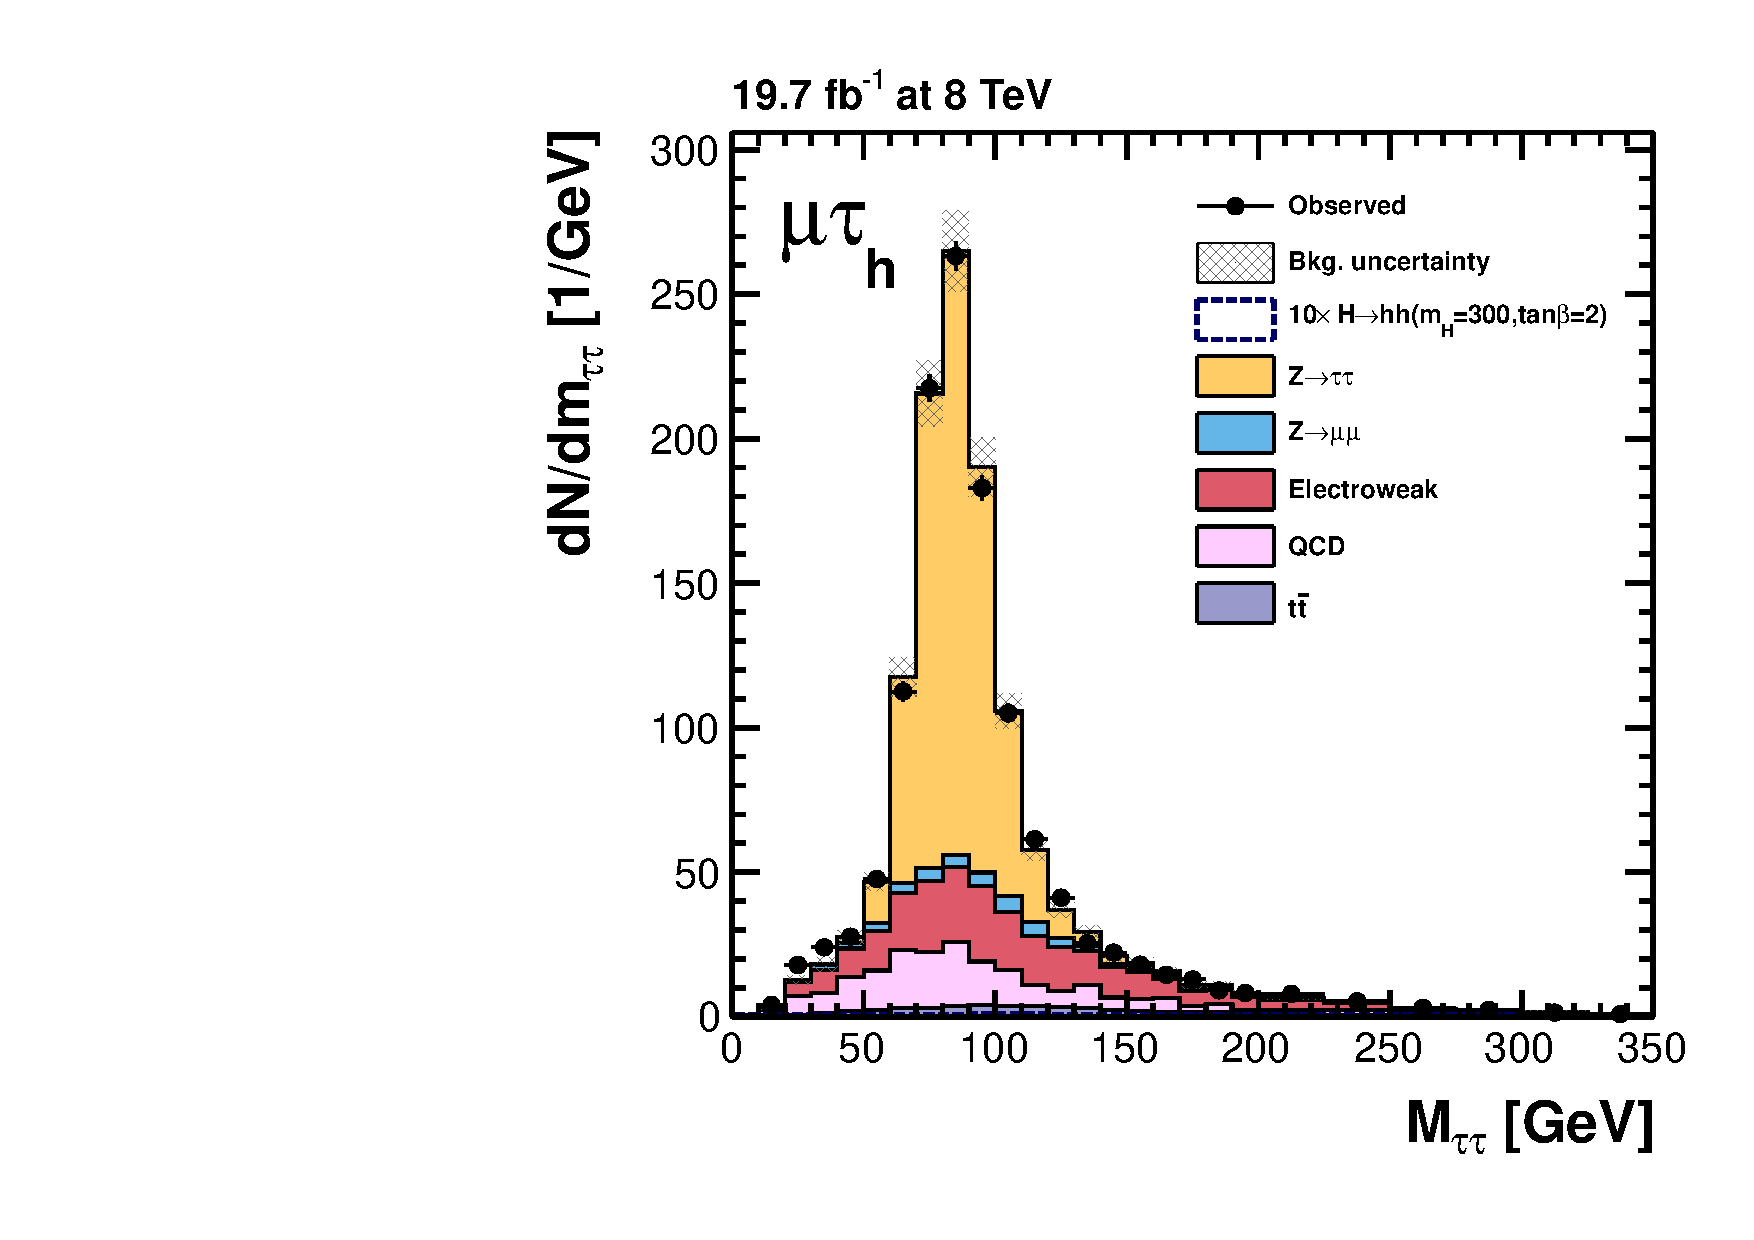
\includegraphics[width=0.5\textwidth]
      {plots/Hhh/m_sv_2jet0tagSF_mt_2012.pdf}}
\subfloat[]{
    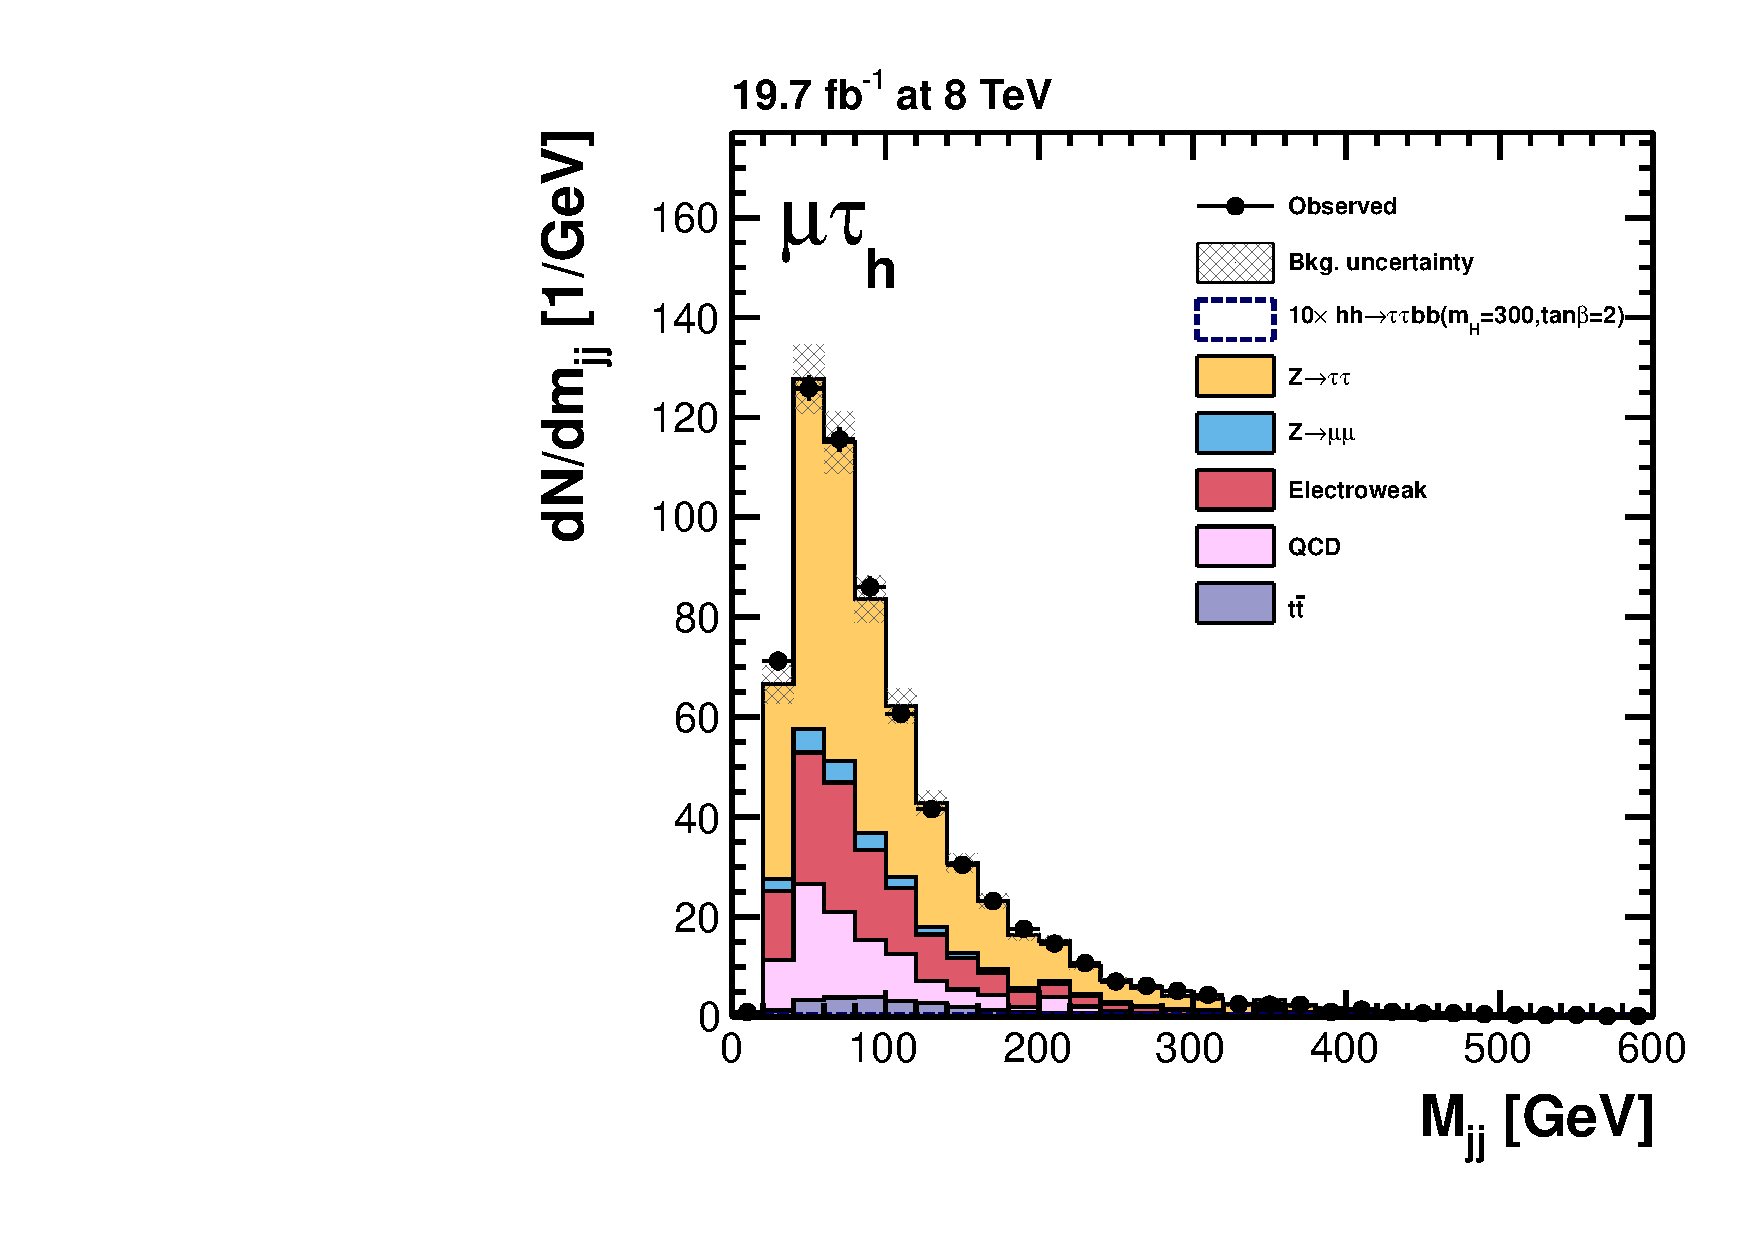
\includegraphics[width=0.5\textwidth] 
      {plots/Hhh/prebjet_mjj_2jet0tagSF_mt_2012.pdf}} 

\subfloat[]{
    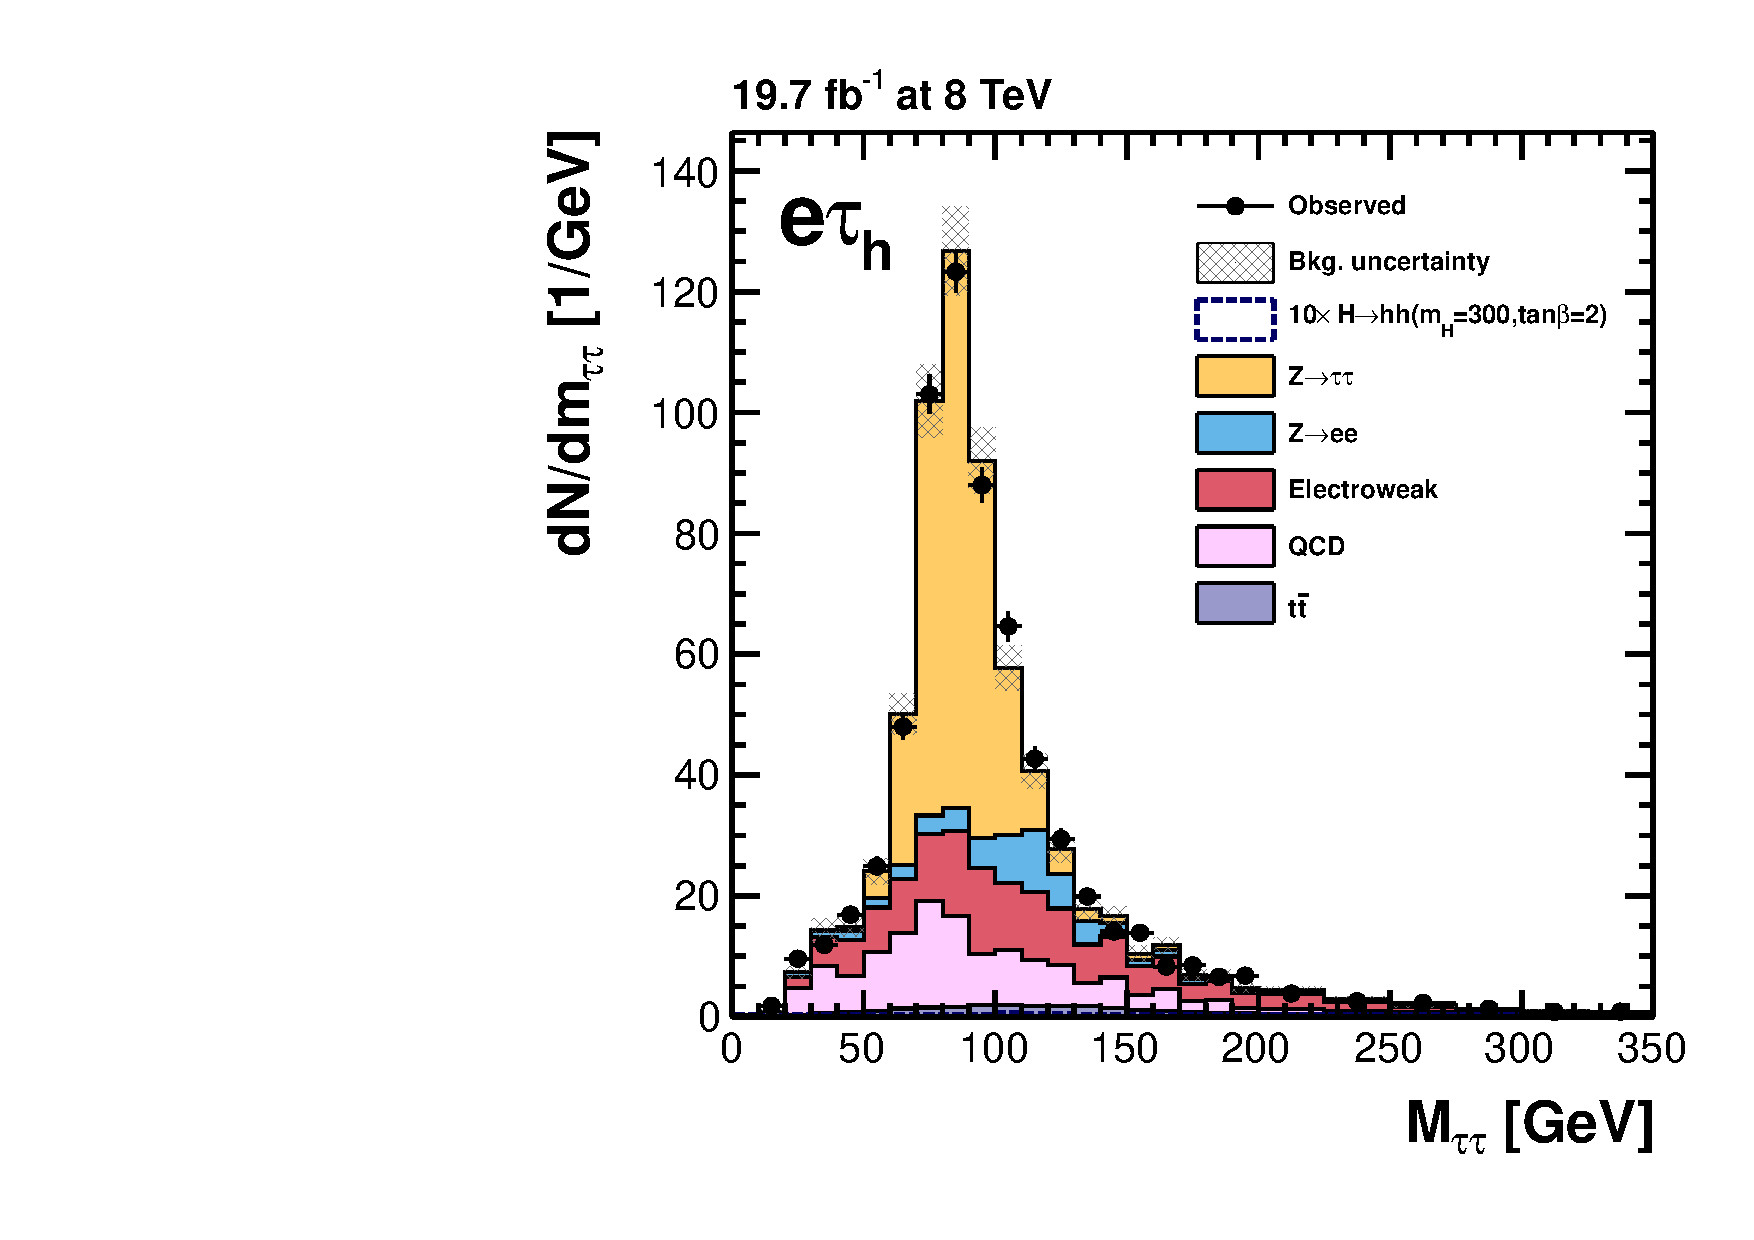
\includegraphics[width=0.5\textwidth]
      {plots/Hhh/m_sv_2jet0tagSF_et_2012.pdf}}
\subfloat[]{
    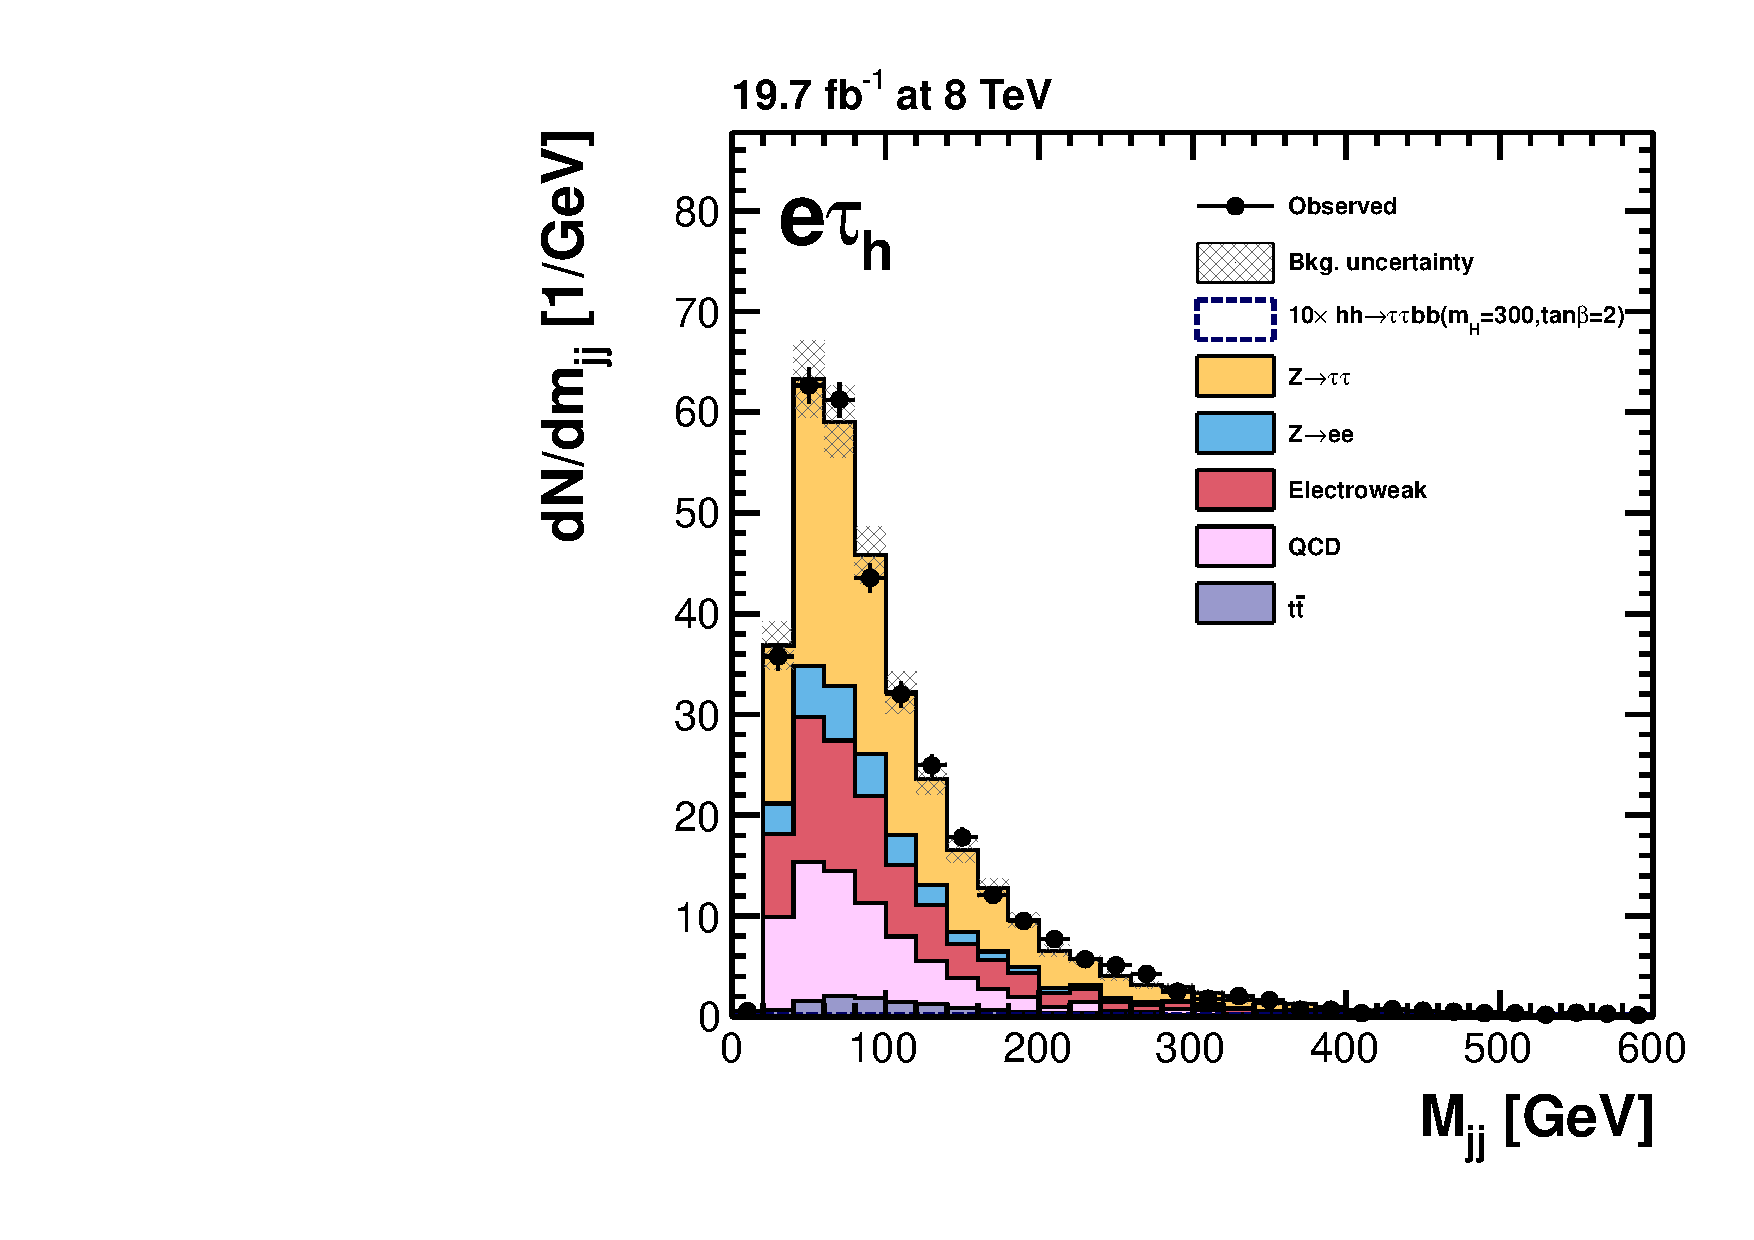
\includegraphics[width=0.5\textwidth] 
      {plots/Hhh/prebjet_mjj_2jet0tagSF_et_2012.pdf}} 
\end{center}
\caption{
Distributions of $m_{\Pgt\Pgt}$ (left) and $m_{\Pqb\Pqb}$ (right) in the $\mutau$ (top) and
$\etau$ (bottom) channels for the 2jet--0tag category. The signal peaks close to $125~\GeV$ in both
variables, motivating the application of cuts in a window around $125~\GeV$ to
select the most signal-like events.}
\label{fig:2jet0tagmttmbb}
\end{figure} 

\begin{figure}
\begin{center}
\subfloat[]{
    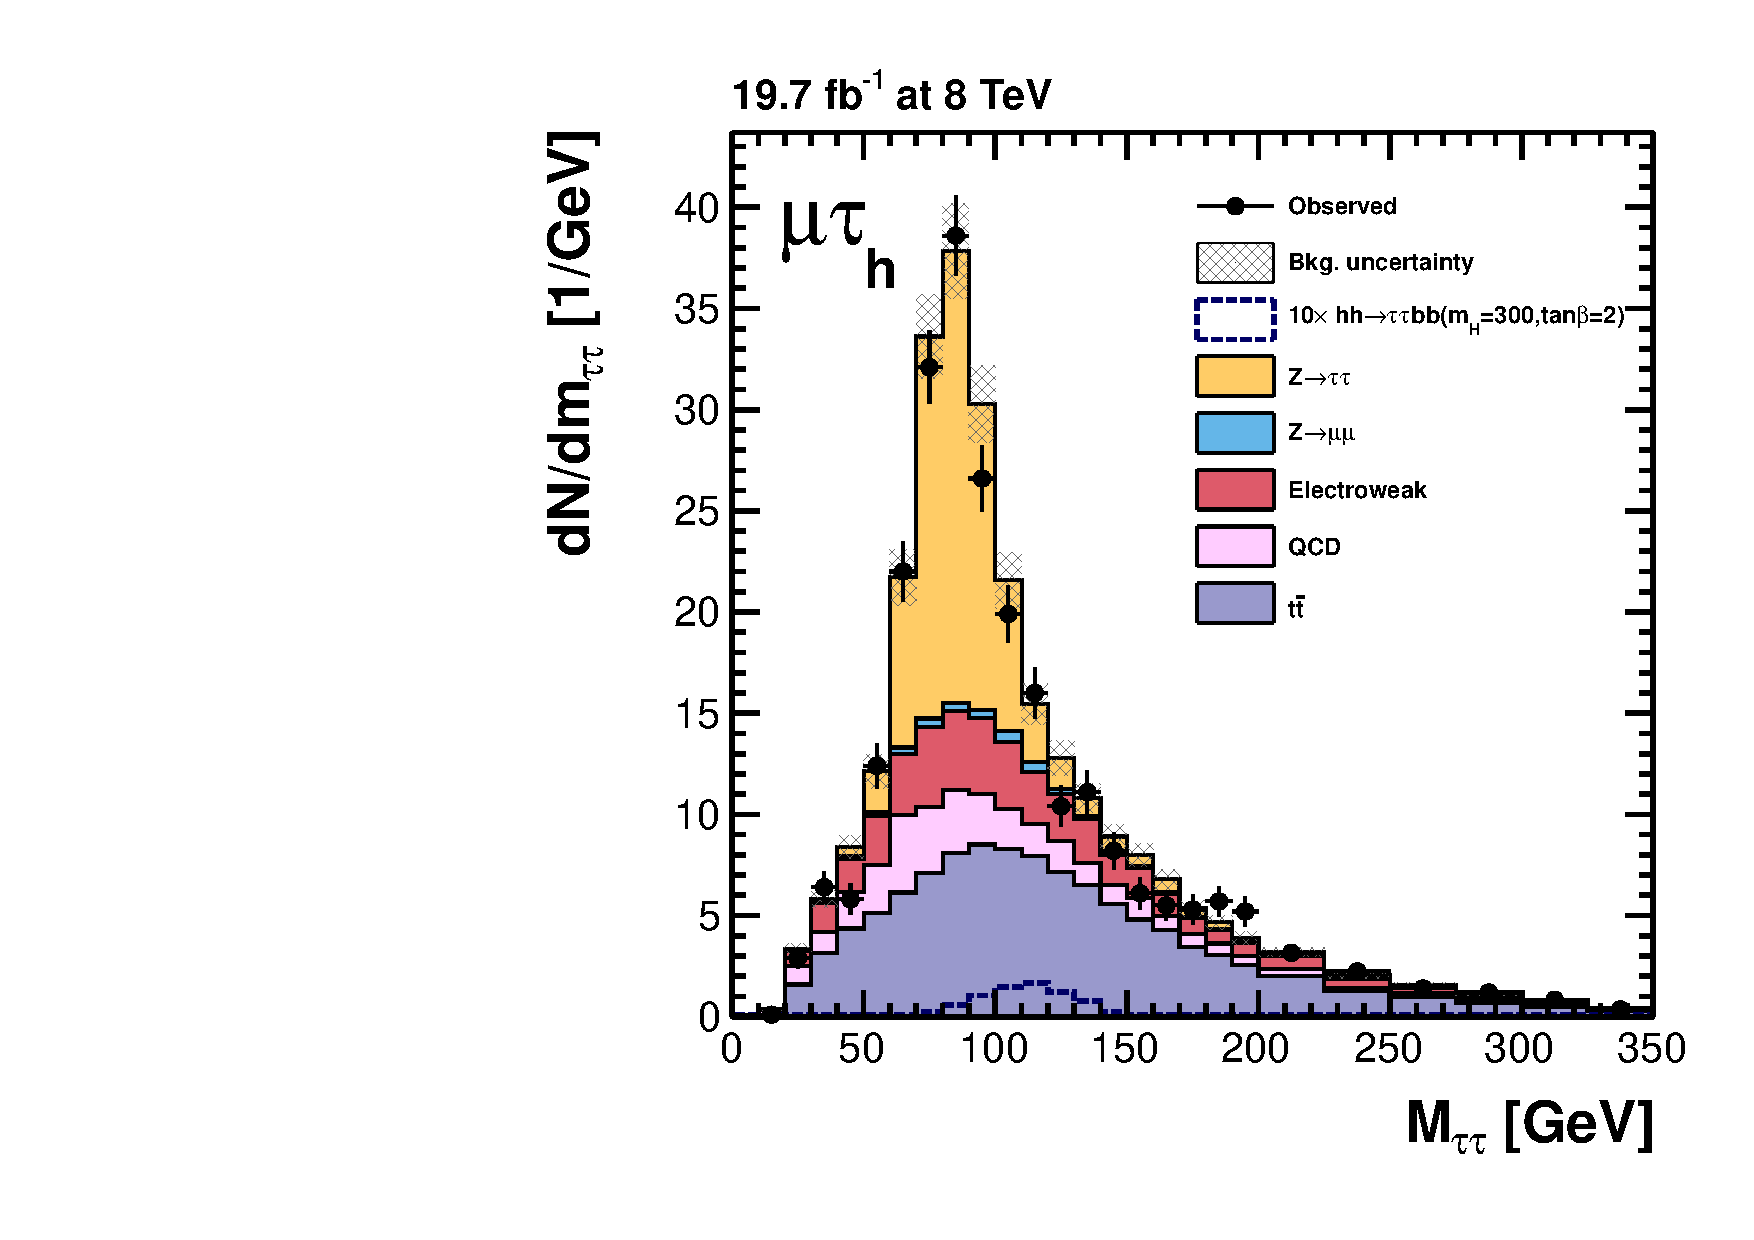
\includegraphics[width=0.5\textwidth]
      {plots/Hhh/m_sv_2jet1tagSF_mt_2012.pdf}}
\subfloat[]{
    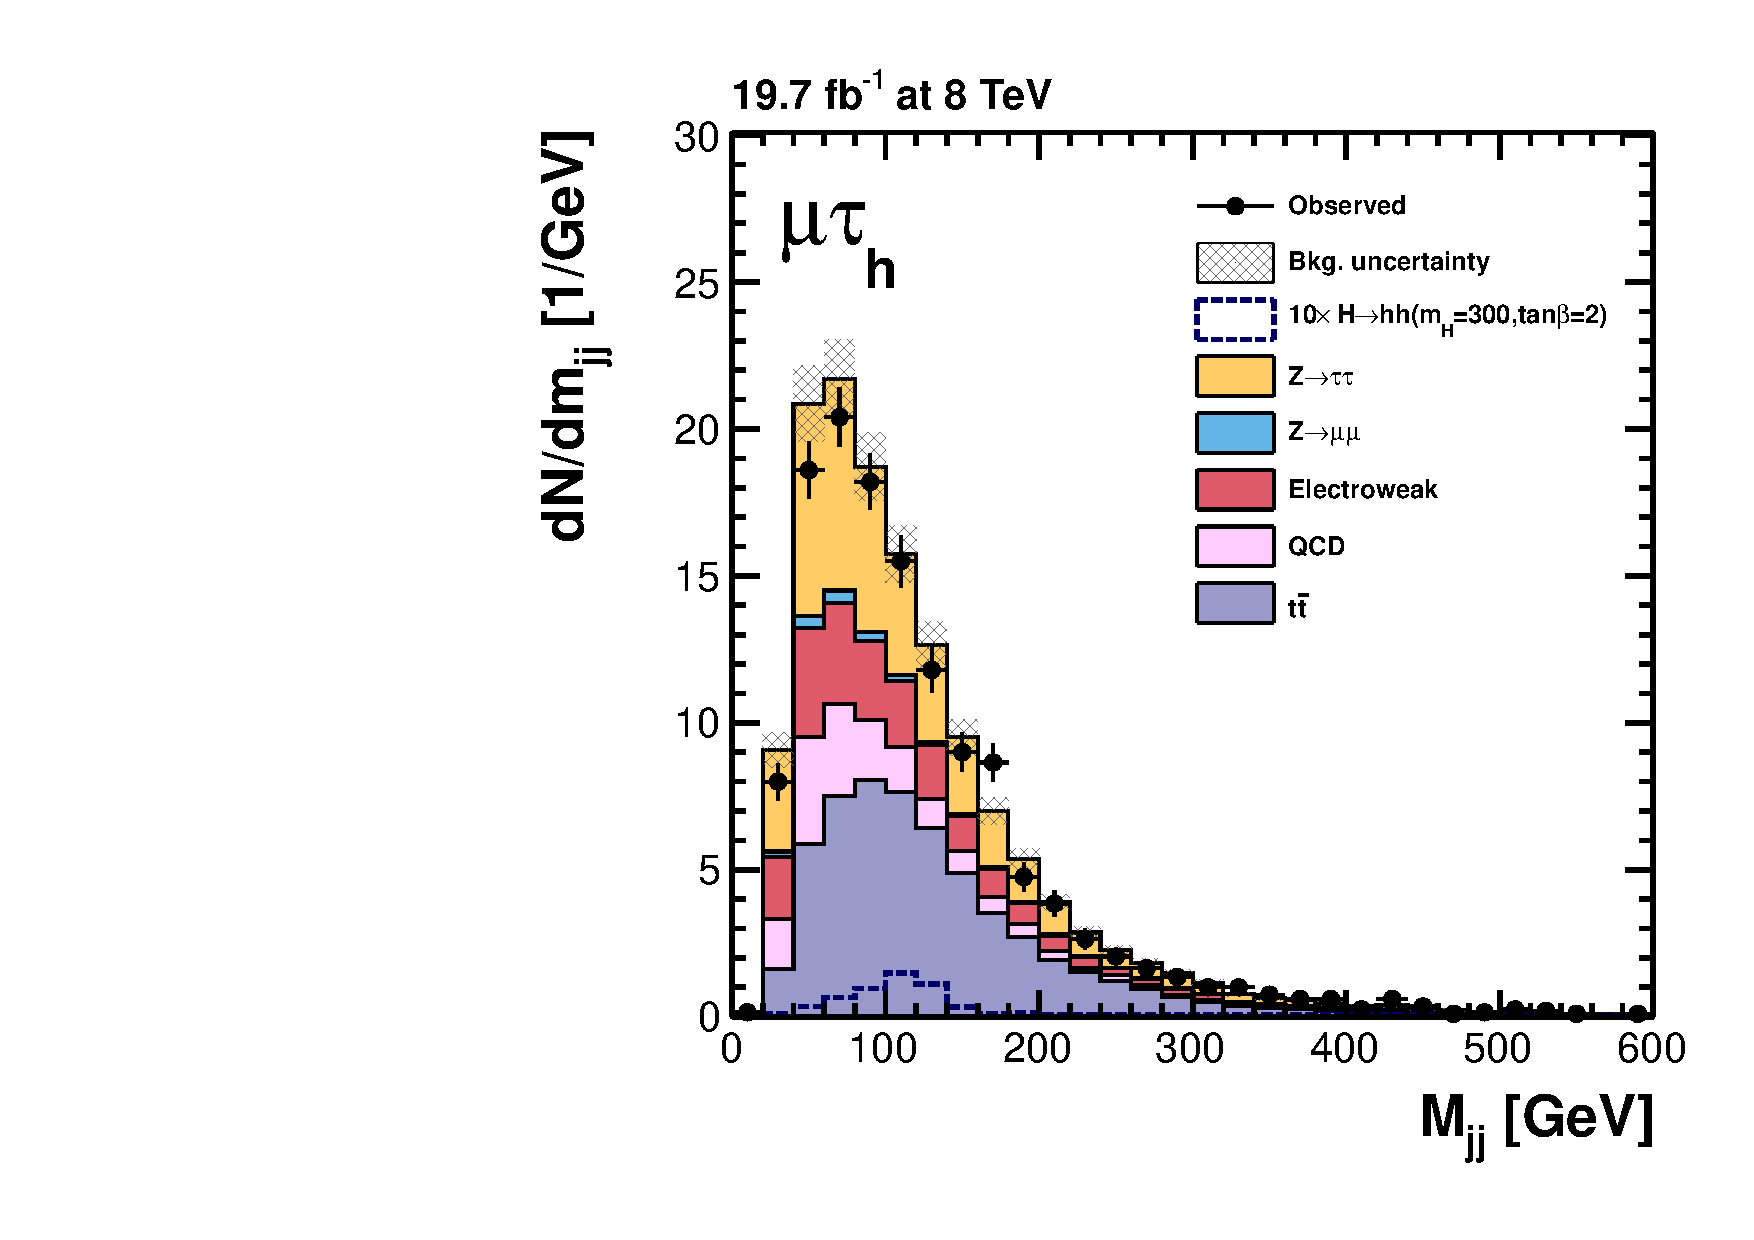
\includegraphics[width=0.5\textwidth] 
      {plots/Hhh/prebjet_mjj_2jet1tagSF_mt_2012.pdf}} 

\subfloat[]{
    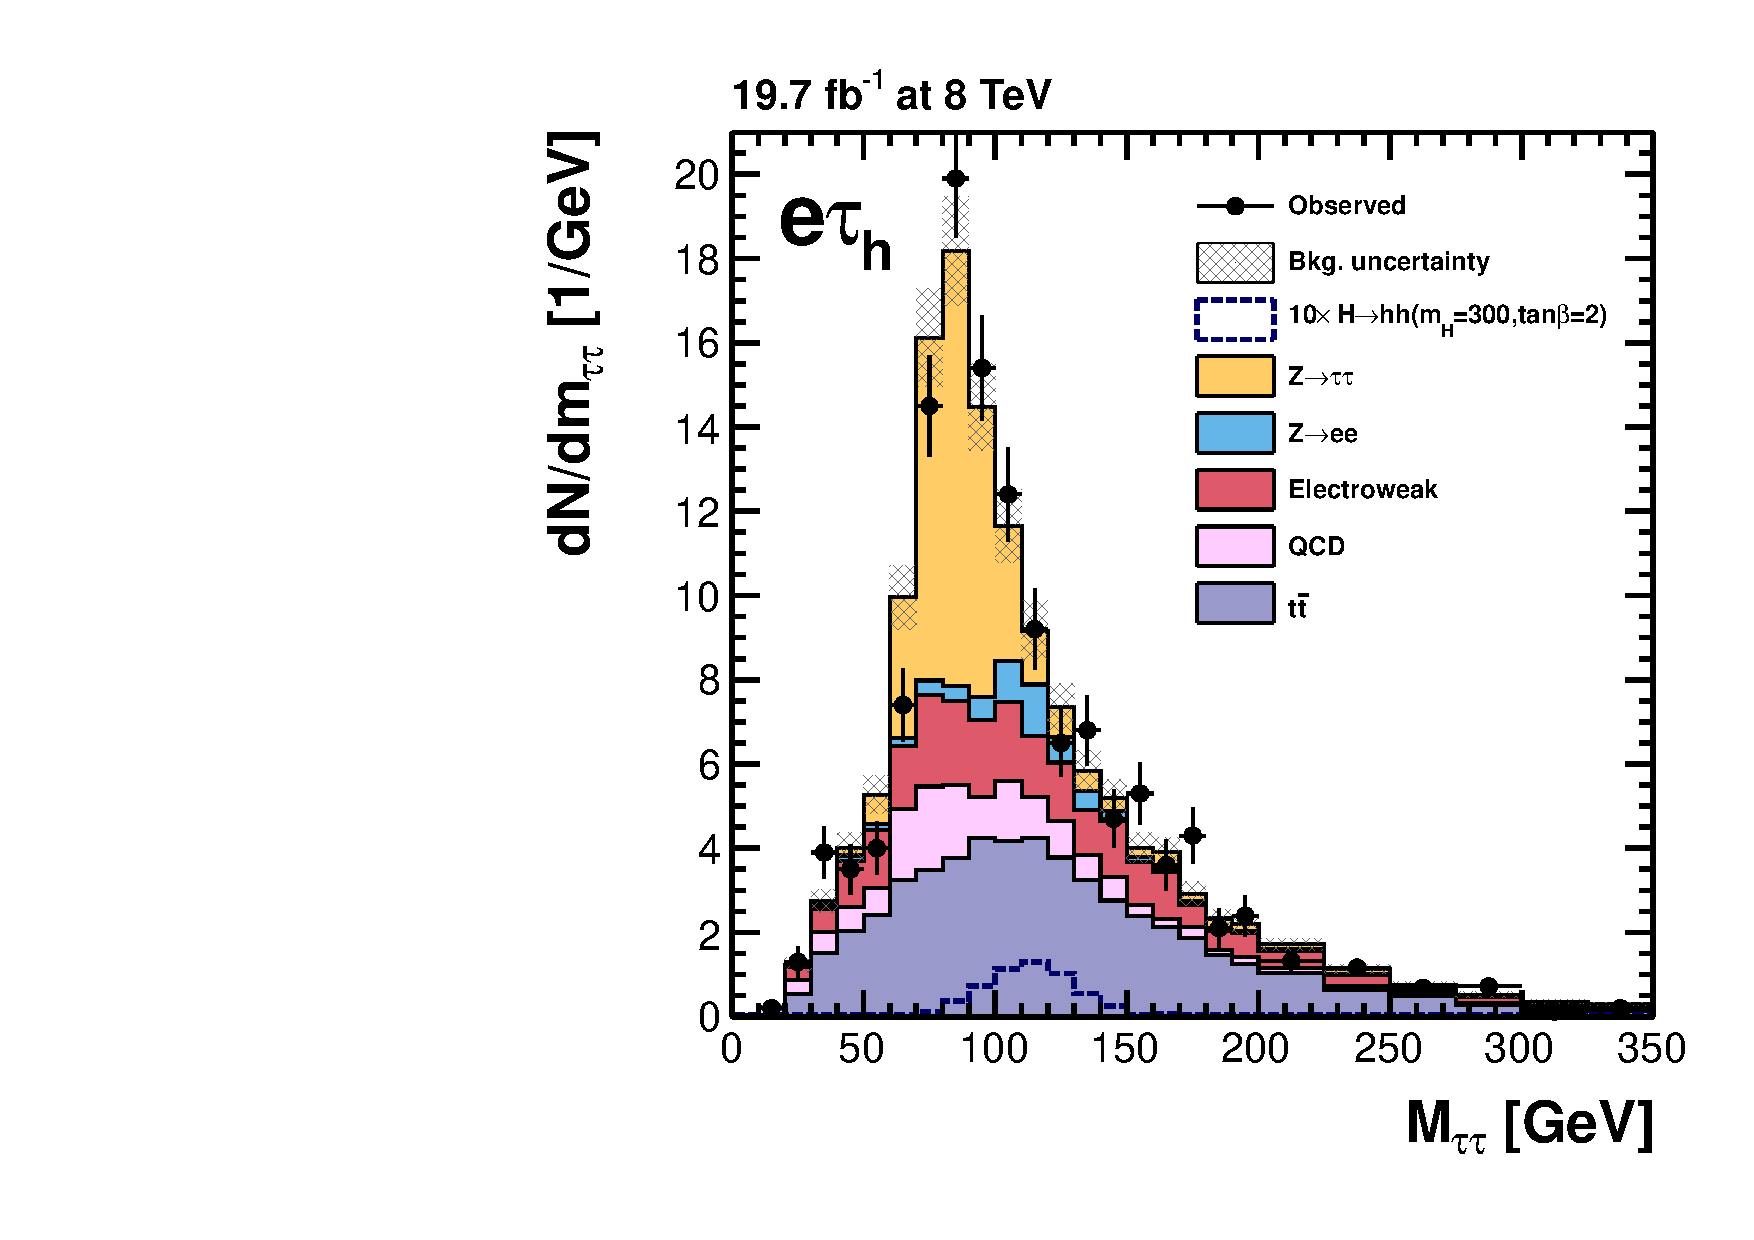
\includegraphics[width=0.5\textwidth]
      {plots/Hhh/m_sv_2jet1tagSF_et_2012.pdf}}
\subfloat[]{
    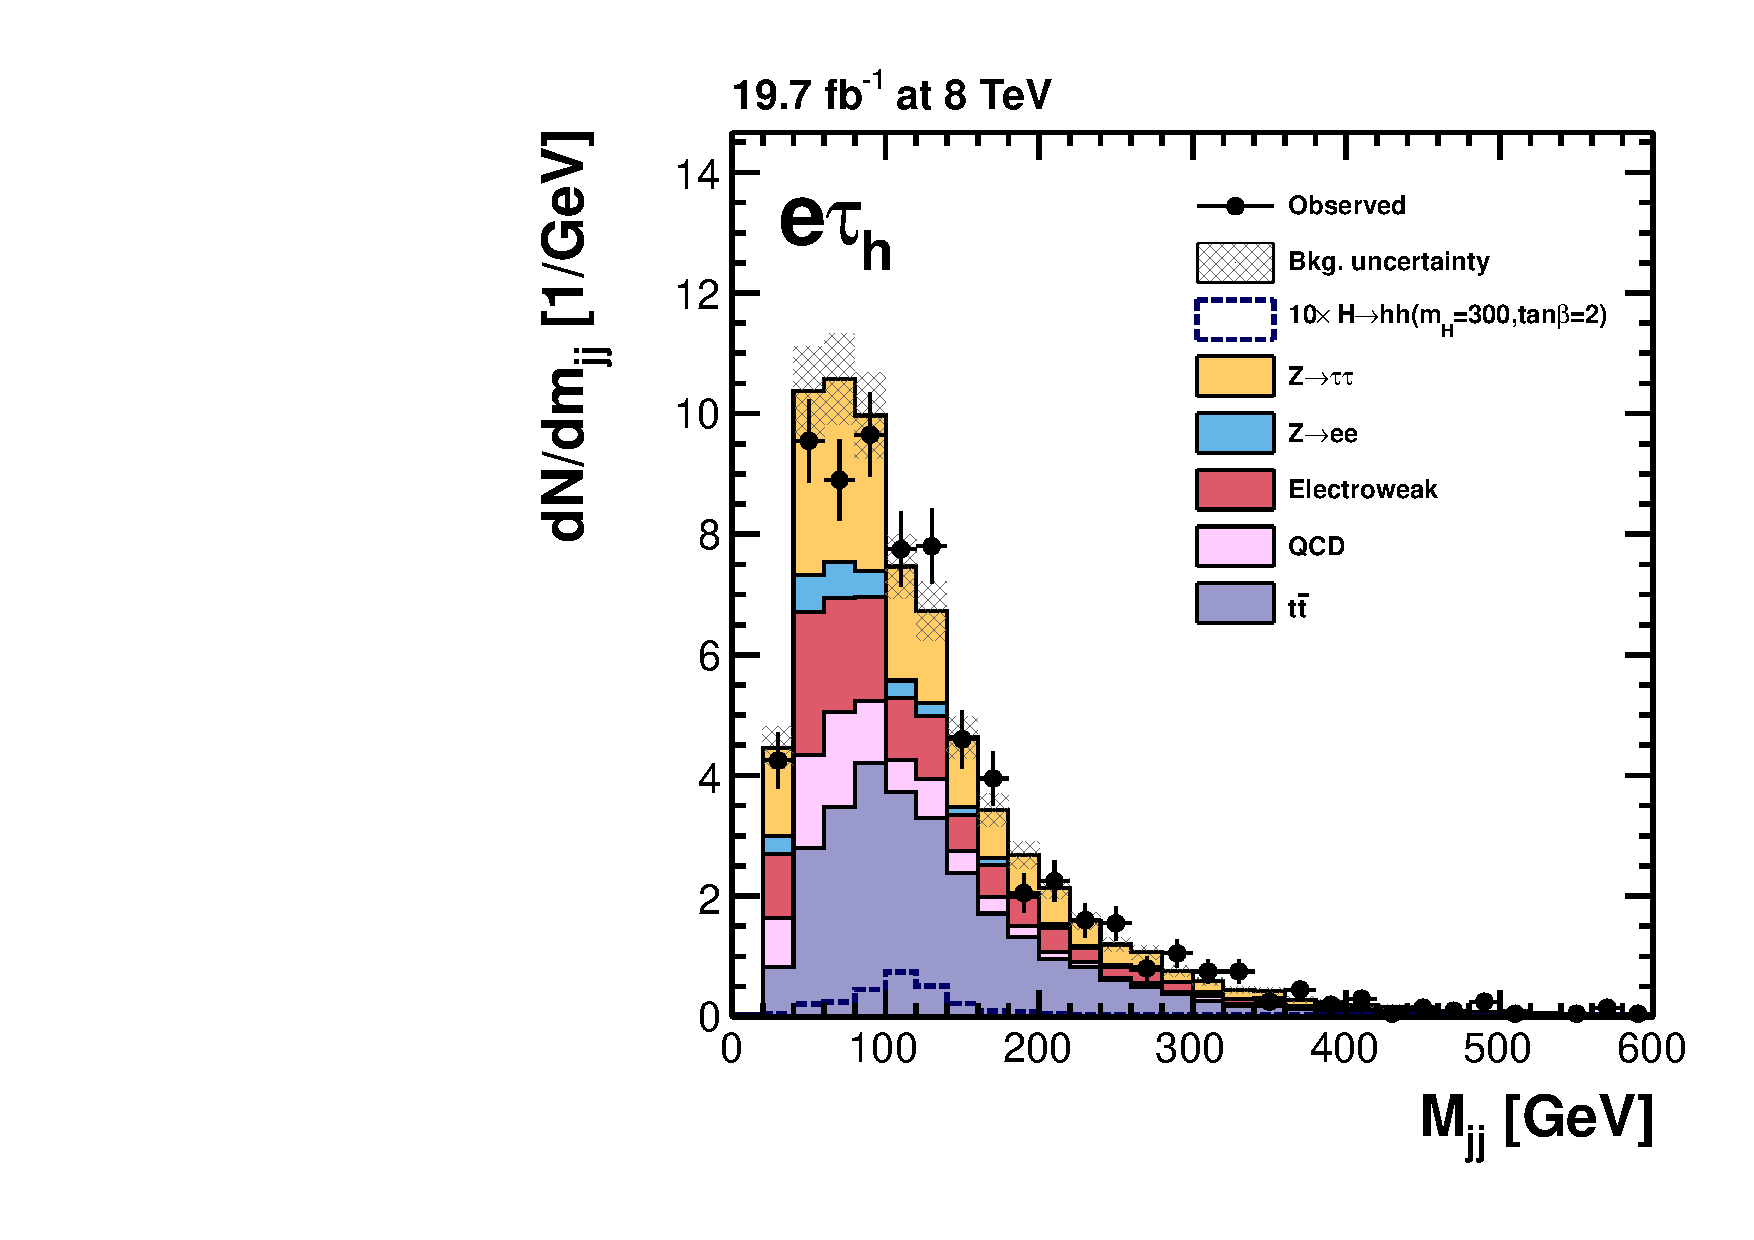
\includegraphics[width=0.5\textwidth] 
      {plots/Hhh/prebjet_mjj_2jet1tagSF_et_2012.pdf}} 
\end{center}
\caption{
Distributions of $m_{\Pgt\Pgt}$ (left) and $m_{\Pqb\Pqb}$ (right) in the $\mutau$ (top) and
$\etau$ (bottom) channels for the 2jet--1tag category. The signal peaks close to $125~\GeV$ in both
variables, motivating the application of cuts in a window around $125~\GeV$ to
select the most signal-like events.}
\label{fig:2jet1tagmttmbb}
\end{figure} 

\begin{figure}
\begin{center}
\subfloat[]{
    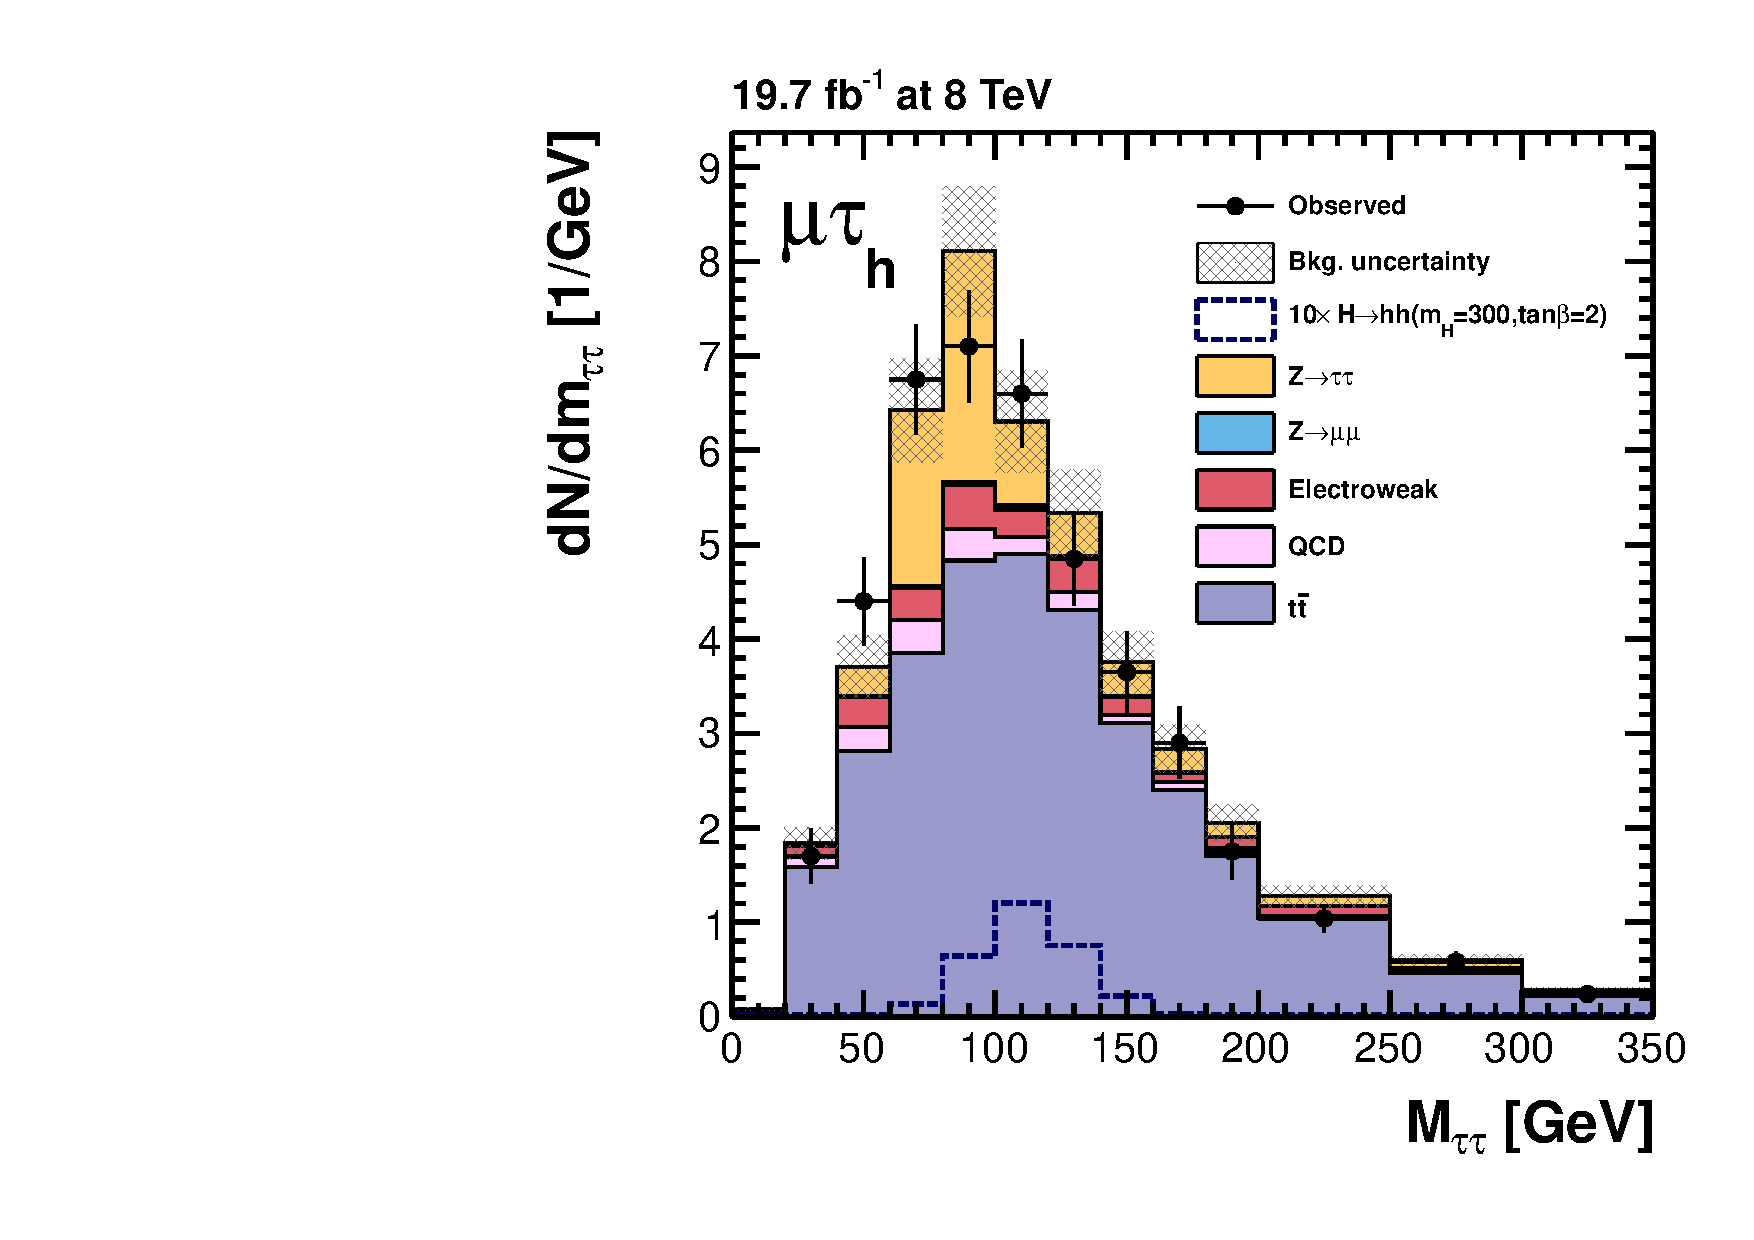
\includegraphics[width=0.5\textwidth]
      {plots/Hhh/m_sv_2jet2tagSF_mt_2012.pdf}}
\subfloat[]{
    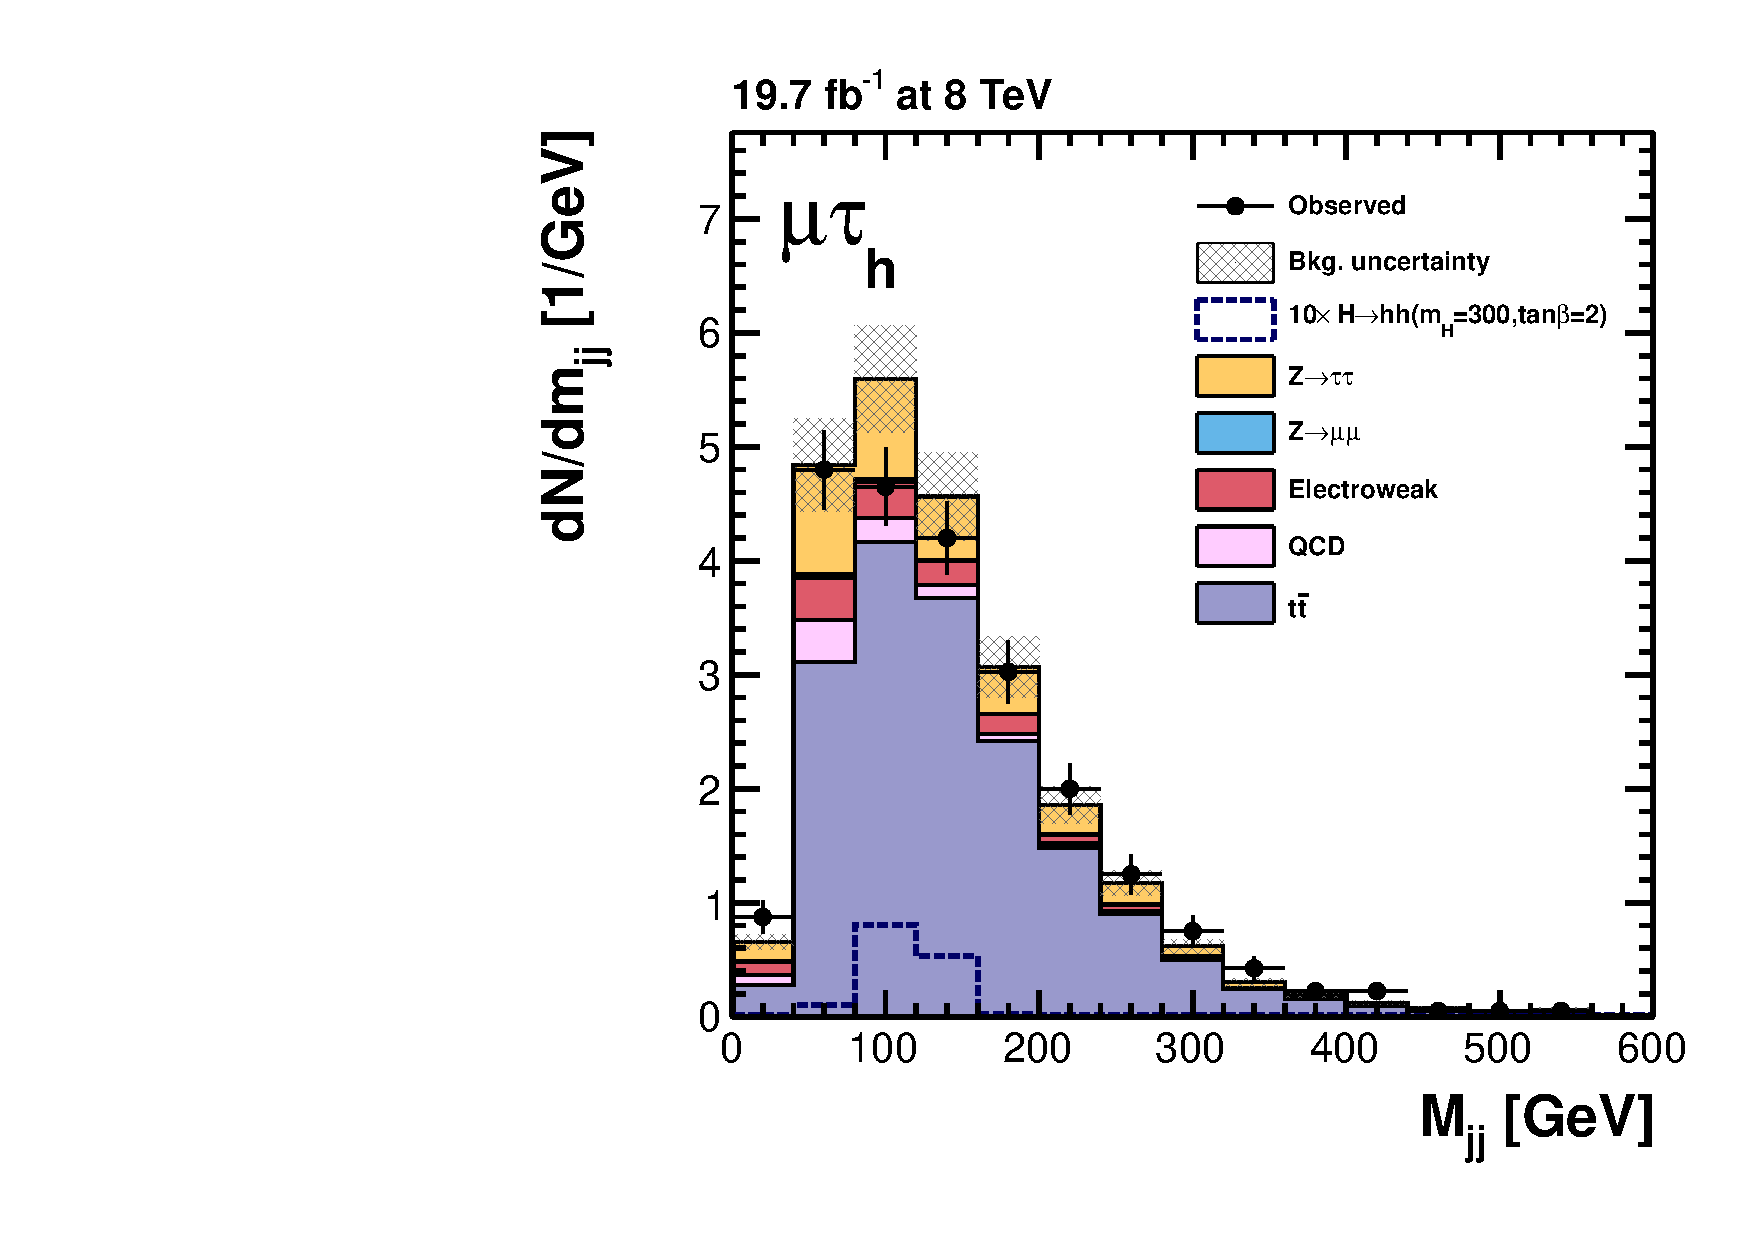
\includegraphics[width=0.5\textwidth] 
      {plots/Hhh/prebjet_mjj_2jet2tagSF_mt_2012.pdf}} 

\subfloat[]{
    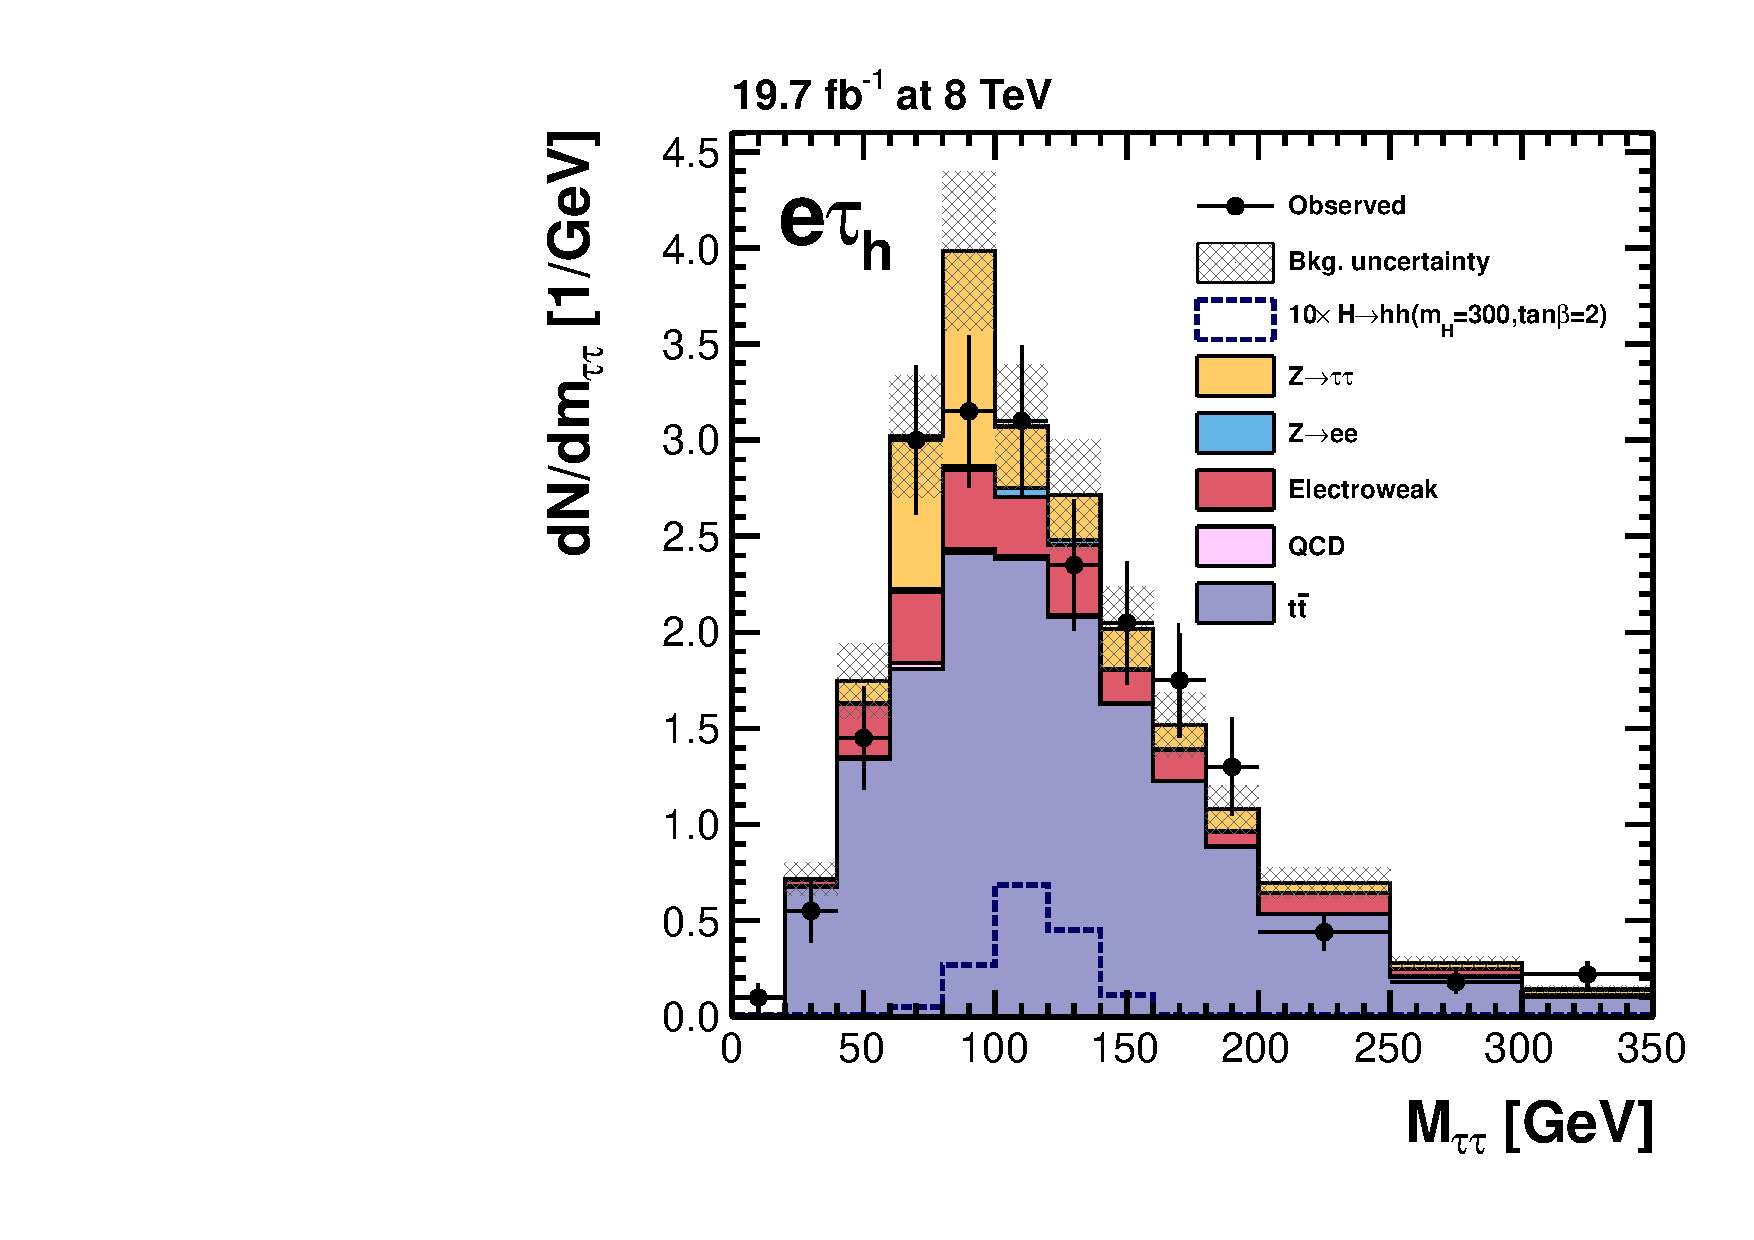
\includegraphics[width=0.5\textwidth]
      {plots/Hhh/m_sv_2jet2tagSF_et_2012.pdf}}
\subfloat[]{
    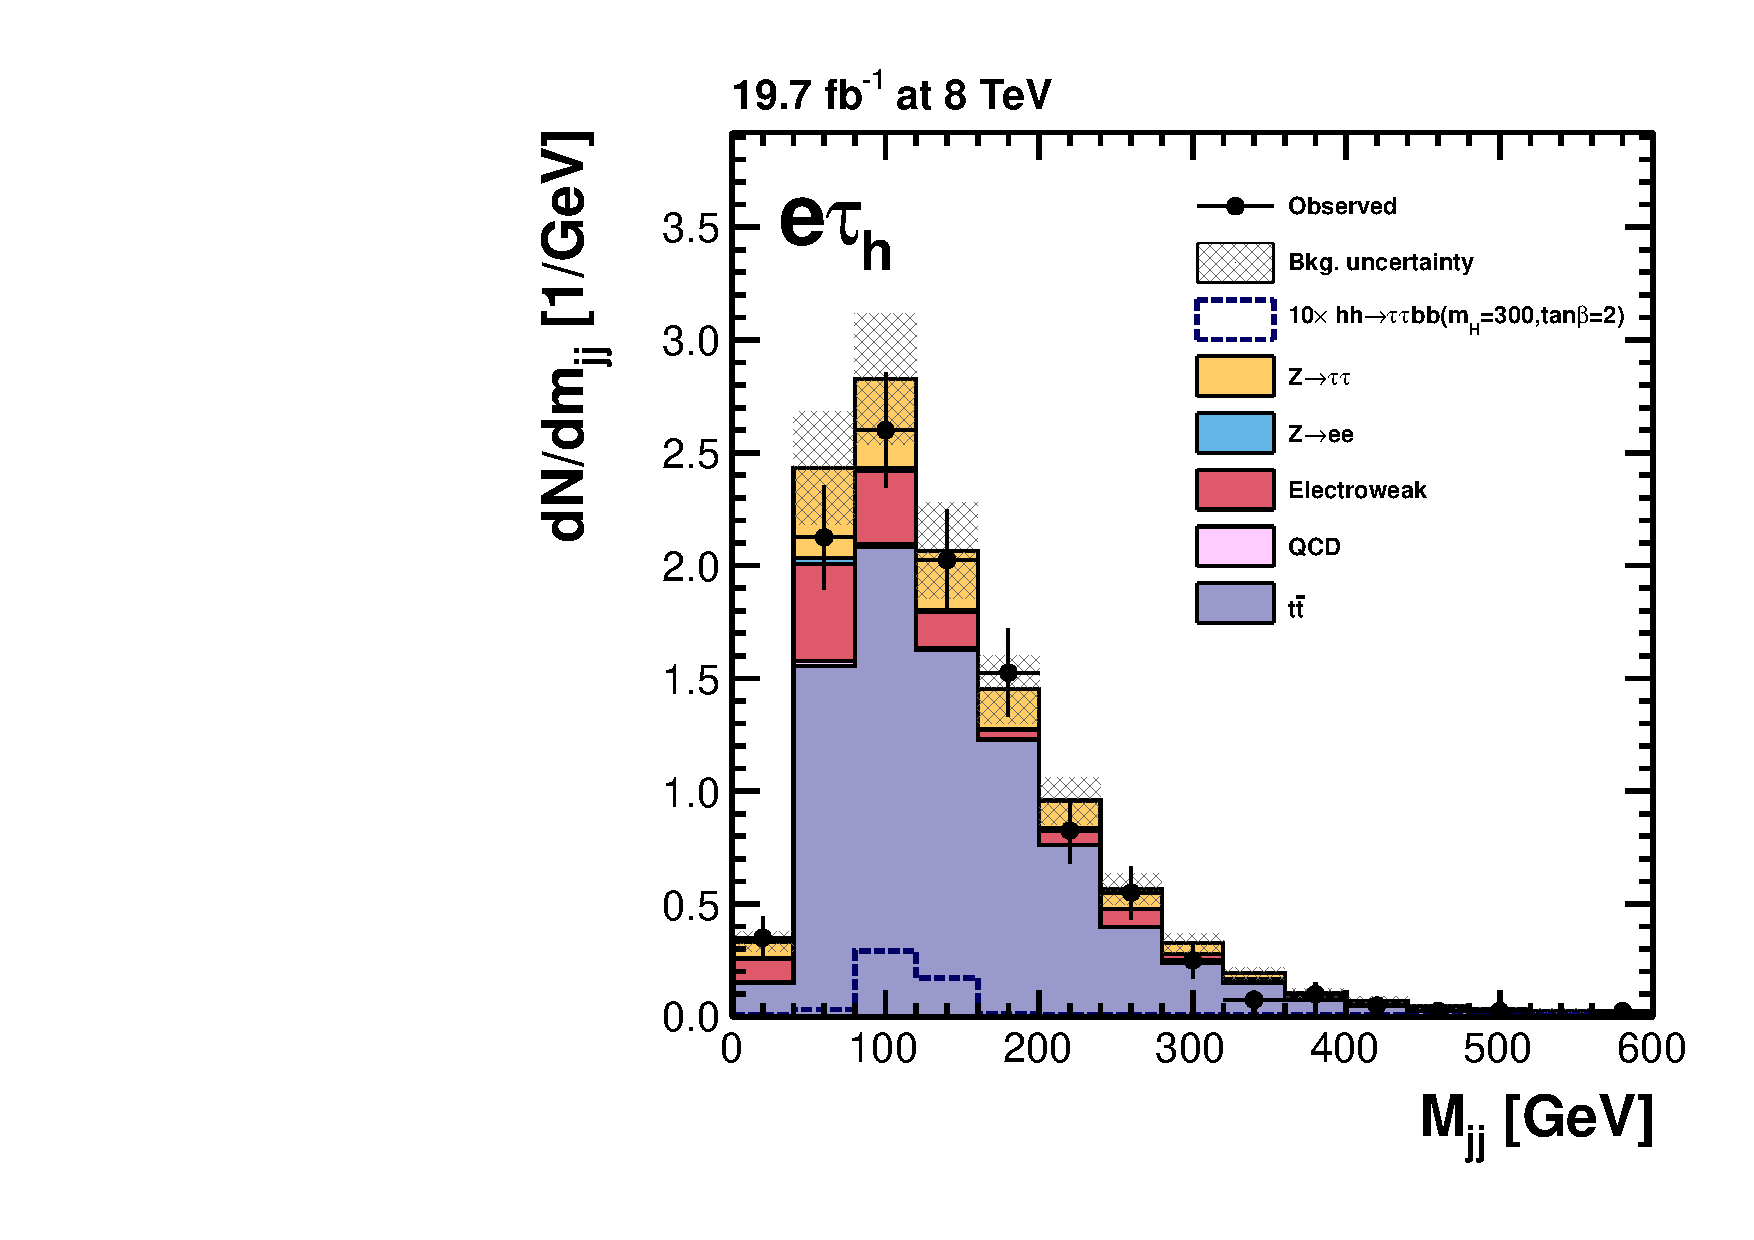
\includegraphics[width=0.5\textwidth] 
      {plots/Hhh/prebjet_mjj_2jet2tagSF_et_2012.pdf}} 
\end{center}
\caption{
Distributions of $m_{\Pgt\Pgt}$ (left) and $m_{\Pqb\Pqb}$ (right) in the $\mutau$ (top) and
$\etau$ (bottom) channels for the 2jet--2tag category. The signal peaks close to $125~\GeV$ in both
variables, motivating the application of cuts in a window around $125~\GeV$ to
select the most signal-like events.}
\label{fig:2jet2tagmttmbb}
\end{figure} 

\section{Kinematic Fitting to extract $M_{H}$}
\label{sec:kinematicfit}

In addition to applying cuts on $m_{bb}$ and $m_{\tau\tau}$, the condition that
both values should be consistent with $125~\GeV$ can be used further in
calculating the reconstructed $M_{\PH}$. This quantity can be reconstructed simply
by combining the visible taus, $\MET$ and the b-jets, denoted by $M_{\tau\tau bb}$.
A better reconstruction is obtained by using the conditions on $m_{bb}$ and
$m_{\tau\tau}$ in a kinematic fit. 

In this method, observables related to the
event kinematics are varied within the measurement uncertainties in order to
find the values which best fulfil a kinematic constraint. In this case, the
variables being varied correspond to the energies of the taus and b-jets and the
kinematic constraints are that $m_{bb} = m_{\tau\tau} = m_{h} = 125~\GeV$. Differences
between the measured value and the constraint are accounted for in a cost
function $\chi^{2}$ which is minimised in the fitting procedure.  

For the b-jets, it is assumed that the reconstructed position in terms of the
angles $\eta_{j}$ and $\phi_{j}$ is known to great accuracy, and the largest
uncertainty is in the measurement of the energy. Thus in the fit, only the
energy of the jets is varied, and the position is kept constant. To first
approximation any uncertainty in energy directly translates to an uncertainty in
momentum related by the quantity $\beta = p/E$, which is assumed to be constant and 
not varied in the fit. The energy of the first b-jet is varied, and then the
energy of the second b-jet can be related to the first using the following
kinematic conditions:

\begin{equation}
m_{H}^{2} = p_{b_{1}}^{2} + p_{b_{2}}^{2,fit} + 2p_{b_{1}}p_{b_{2}}^{fit} 
          = m_{b_{1}}^{2} + \frac{E_{b_{2}}^{2,fit}}{\gamma_{b_{2}}^{2}} +
          2E_{b_{1}}E_{b_{2}}^{fit}\left(\underbrace{1-\vec{\beta}_{b_{1}}\vec{\beta}_{b_{2}}}_{A}\right),   
\label{eq:bjetkinfit}         
\end{equation}

where $\gamma_{b_{1,2}} = 1/\sqrt{1-\beta_{b_{1,2}}^{2}}$. The term $A$ is
assumed to be constant and hence can be derived from the pre-fit event
kinematics as:

\begin{equation}
A = \frac{m_{b_{1}b_{2}}^{2} - m_{b_{1}}^{2} - m_{b_{2}}^{2}}{2E_{b_{1}}E_{b_{2}}} , 
\end{equation}

which allows equation \ref{eq:bjetkinfit} to be reduced to:

\begin{equation}
E_{b_{2}}^{fit} = E_{b_{1}}A\gamma_{b_{2}}^{2}\left(-1 + \sqrt{1 +
\frac{m_{h}^{2} -
m_{b_{1}^{2}}}{\left(E_{b_{1}}A\gamma_{b_{2}}\right)^{2}}}\right) .
\label{eq:bjetrelation}
\end{equation}

A $\chi^{2}$ quantity can then be constructed to quantify how much the fit has
modified the b-jet energy as:

\begin{equation}
\chi_{b_{1,2}}^{2} = \frac{E_{b_{1,2}}^{fit} -
E_{b_{1,2}}^{meas}}{\sigma_{b_{1,2}}}
\end{equation}

where $E_{b_{1,2}}^{meas}$ is the measured b-jet energy and $\sigma_{b_{1,2}}$
is the b-jet energy resolution. The value of $\sigma_{b_{1,2}}$ is estimated
using a \ac{MC} sample in different bins of $\eta$ and $\pt$. 

The $\Pgt$s are treated in a slightly different way in the fit due to the $\MET$
associated with their decays. It is assumed that the collinear approximation
holds such that the visible products are produced in the same direction as the
original tau. This direction is assumed to be known to a high degree of
accuracy, as in the case of the b-jets, and so is not varied in the fit. Thus as
in the case of the b-jets, only the energy of one $\Pgt$ is free in the fit, and
the energy of the other $\Pgt$ can be related to the first in an analogous way
to in equation \ref{eq:bjetrelation}. The mass of either $\Pgt$ lepton is kept
constant at $m_{\Pgt}$.  

In order to find the correct $\Pgt$ energies, additional constraints are put on
the event using the $\MET$ to enforce that the heavy Higgs recoil from the fit
is close to the reconstructed recoil. The recoil from the fit can be defined as:
%check this equation - should they all be p_T?
\begin{equation}
\vec{p}_{\text{T},\text{recoil}}^{\text{~~fit}} = -
\vec{p}_{\text{T},b_{1}}^{\text{~~fit}} -
\vec{p}_{\text{T},b_{2}}^{\text{~~fit}} -
\vec{p}_{\text{T},\Pgt_{1}}^{\text{~~fit}} - \vec{p}_{\text{T},\Pgt_{2}}^{\text{~~fit}} = -
\vec{p}_{\text{T},\text{H}}^{\text{~~fit}} ,
\end{equation}

and the measured recoil as:

\begin{equation}
\vec{p}_{\text{T},\text{recoil}}^{\text{~~meas}} = -
\vec{p}_{\text{T},\text{miss}}^{\text{~~meas}} -
\vec{p}_{\text{T},b_{1}}^{\text{~~meas}} - \vec{p}_{\text{T},b_{2}}^{\text{~~meas}} -
\vec{p}_{\text{T},\Pgt_{1}^{\text{vis}}}^{\text{~~meas}} -
\vec{p}_{\text{T},\Pgt_{2}^{\text{vis}}}^{\text{~~meas}} = -
\vec{p}_{\text{T},\text{H}}^{\text{~~meas}}
\end{equation}

The $\chi^{2}$ term corresponding to the agreement between these two quantities
can be constructed as:

\begin{equation}
\chi_{\text{recoil}}^{2} = \vec{p}_{\text{T},\text{recoil}}^{\text{~~res},\text{T}} \cdot
\text{COV}_{\text{recoil}}^{-1} \cdot
\vec{p}_{\text{T},\text{recoil}}^{\text{~~res}} ,  
\end{equation}

where $\vec{p}_{\text{T},\text{recoil}}^{\text{~~res}}$ is the residuum vector between
$\vec{p}_{\text{T},\text{recoil}}^{\text{~~fit}}$
and $\vec{p}_{\text{T},\text{recoil}}^{\text{~~meas}}$, and
$\vec{p}_{\text{T},\text{recoil}}^{\text{~~res},\text{T}}$ indicates the
transpose. The covariance matrix of the recoil vector is estimated from
the covariance matrix of the $\vec{p}_{\text{T},\text{miss}}$ and the uncertainties of the b-jets as
follows:

\begin{equation}
\text{COV}_{\text{recoil}} = \text{COV}_{\vec{p}_{T,miss}} - \text{COV}_{b_{1}} -
\text{COV}_{b_{2}} .
\end{equation}

The covariance matrices of the b-jets can be expressed entirely in terms of the
b-jet energy/momentum and position. Hence with inputs of the values and
covariance matrix of the missing tranverse momentum this component of the
$\chi^{2}$ is entirely specified. 

The total $\chi^{2}$ to be minimised by the fit is then given by:

\begin{equation}
\chi^{2}= \chi_{b_{1}}^{2} + \chi_{b_{2}}^{2} + \chi_{recoil}^{2},
\end{equation}

which is a two dimensional function in variables $E_{b_{1}}$ and $E_{\Pgt_{1}}$.

The output of the kinematic fit is the 4-vector of each of the taus and b-jets,
with the energy and momentum corrected by the result of the fit. Figure
\ref{fig:kinfitvsmttbb}
shows the difference between the heavy Higgs mass as reconstructed by
$M_{\Pgt\Pgt \Pqb\Pqb}$ and from the kinematic fit, denoted $M_{\PH}^{kinfit}$,
in signal events with $m_{\PH}=300~\GeV$. It can
be seen that both the mean and resolution of $M_{\PH}$ is greatly improved in
signal.

\begin{figure}
\begin{center}
    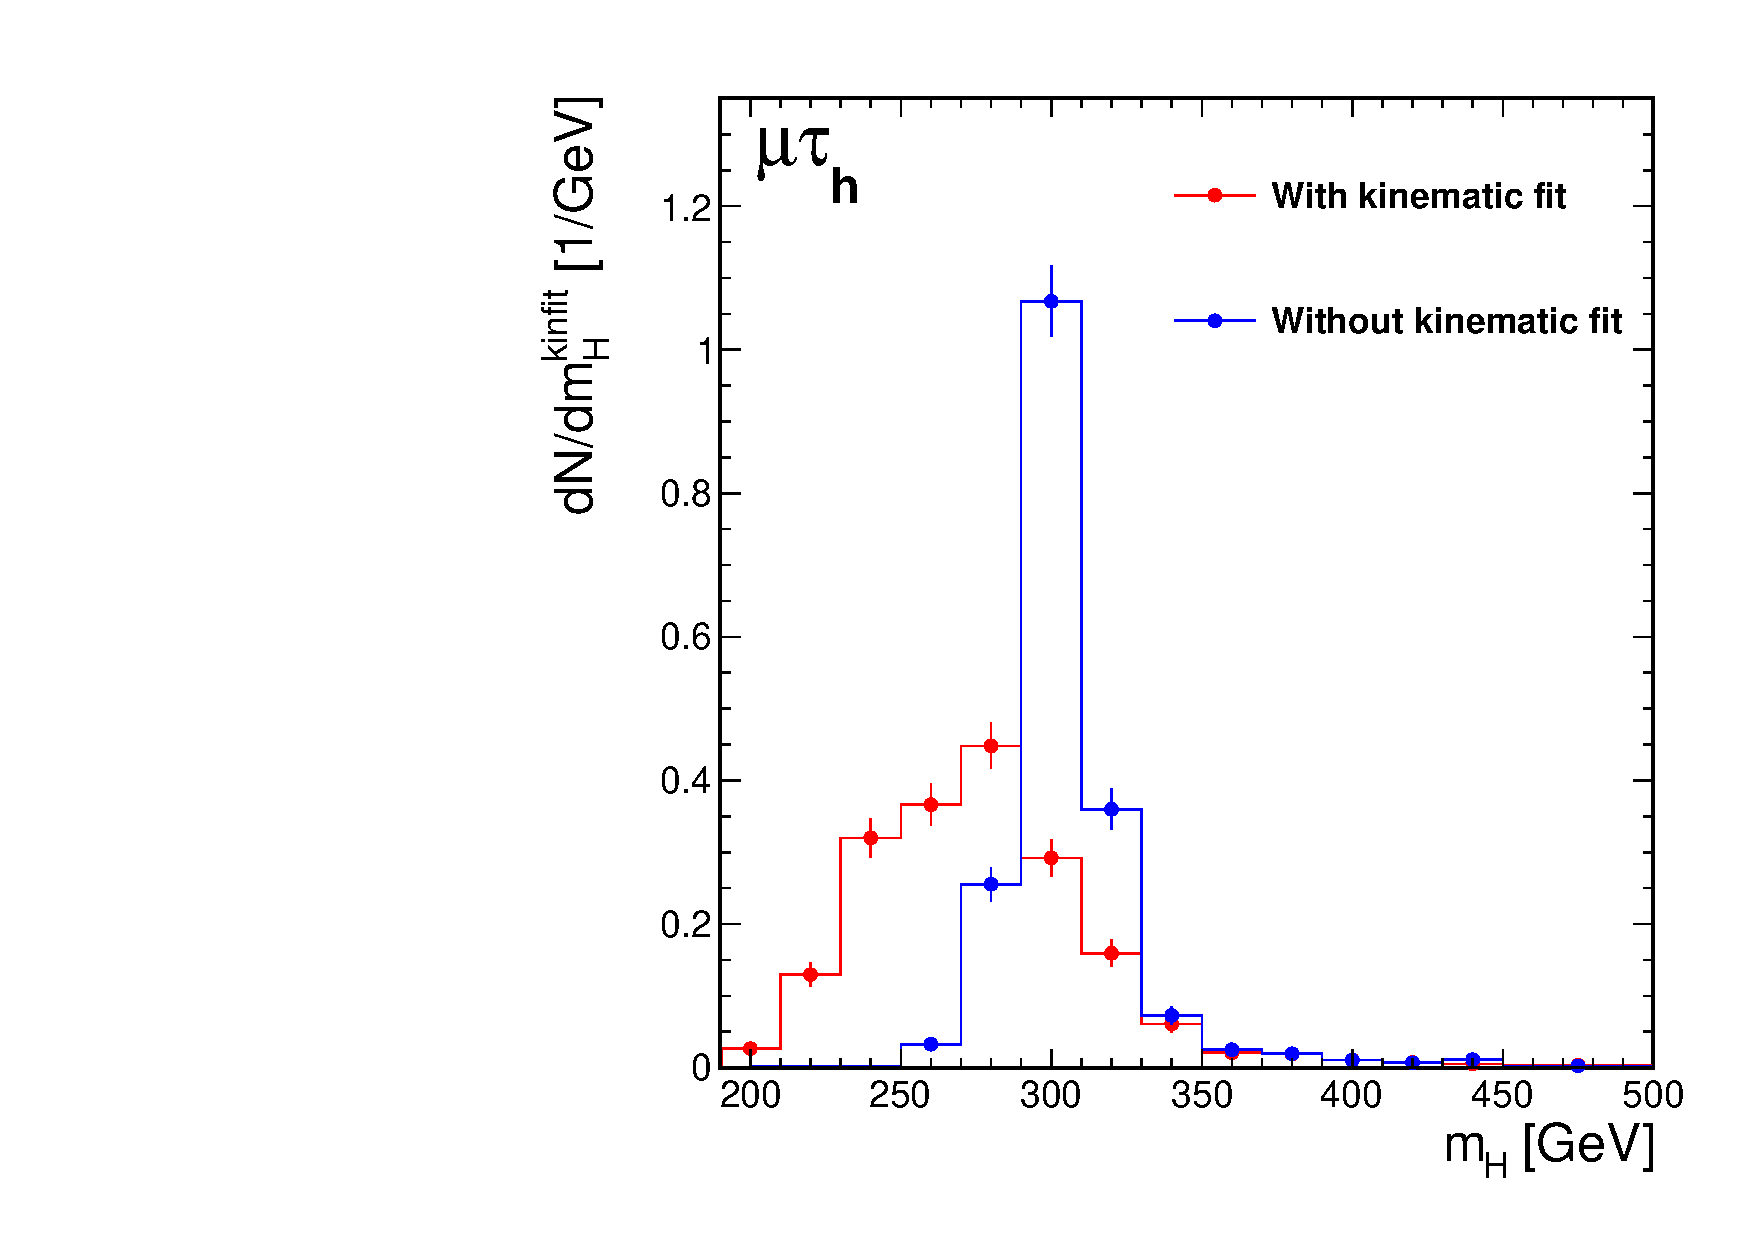
\includegraphics[width=0.5\textwidth]
      {plots/Hhh/m_H_kinfit_vs_mttbb_2jet2tagSFMassCuts_mt_ggHTohh300.pdf}

\end{center}
\caption{
Four body mass of the candidate \PH in $\PH\to\Ph\Ph$ signal events with
$m_{\PH}=300~\GeV$, as reconstructed using a simple sum of the
individual components (without kinematic fit) or using a kinematic fit as
described in the text. Shown for events in the 2jet--2tag category of the
$\mutau$ channel.}
\label{fig:kinfitvsmttbb}
\end{figure} 


\begin{figure}
\begin{center}
\subfloat[]{
    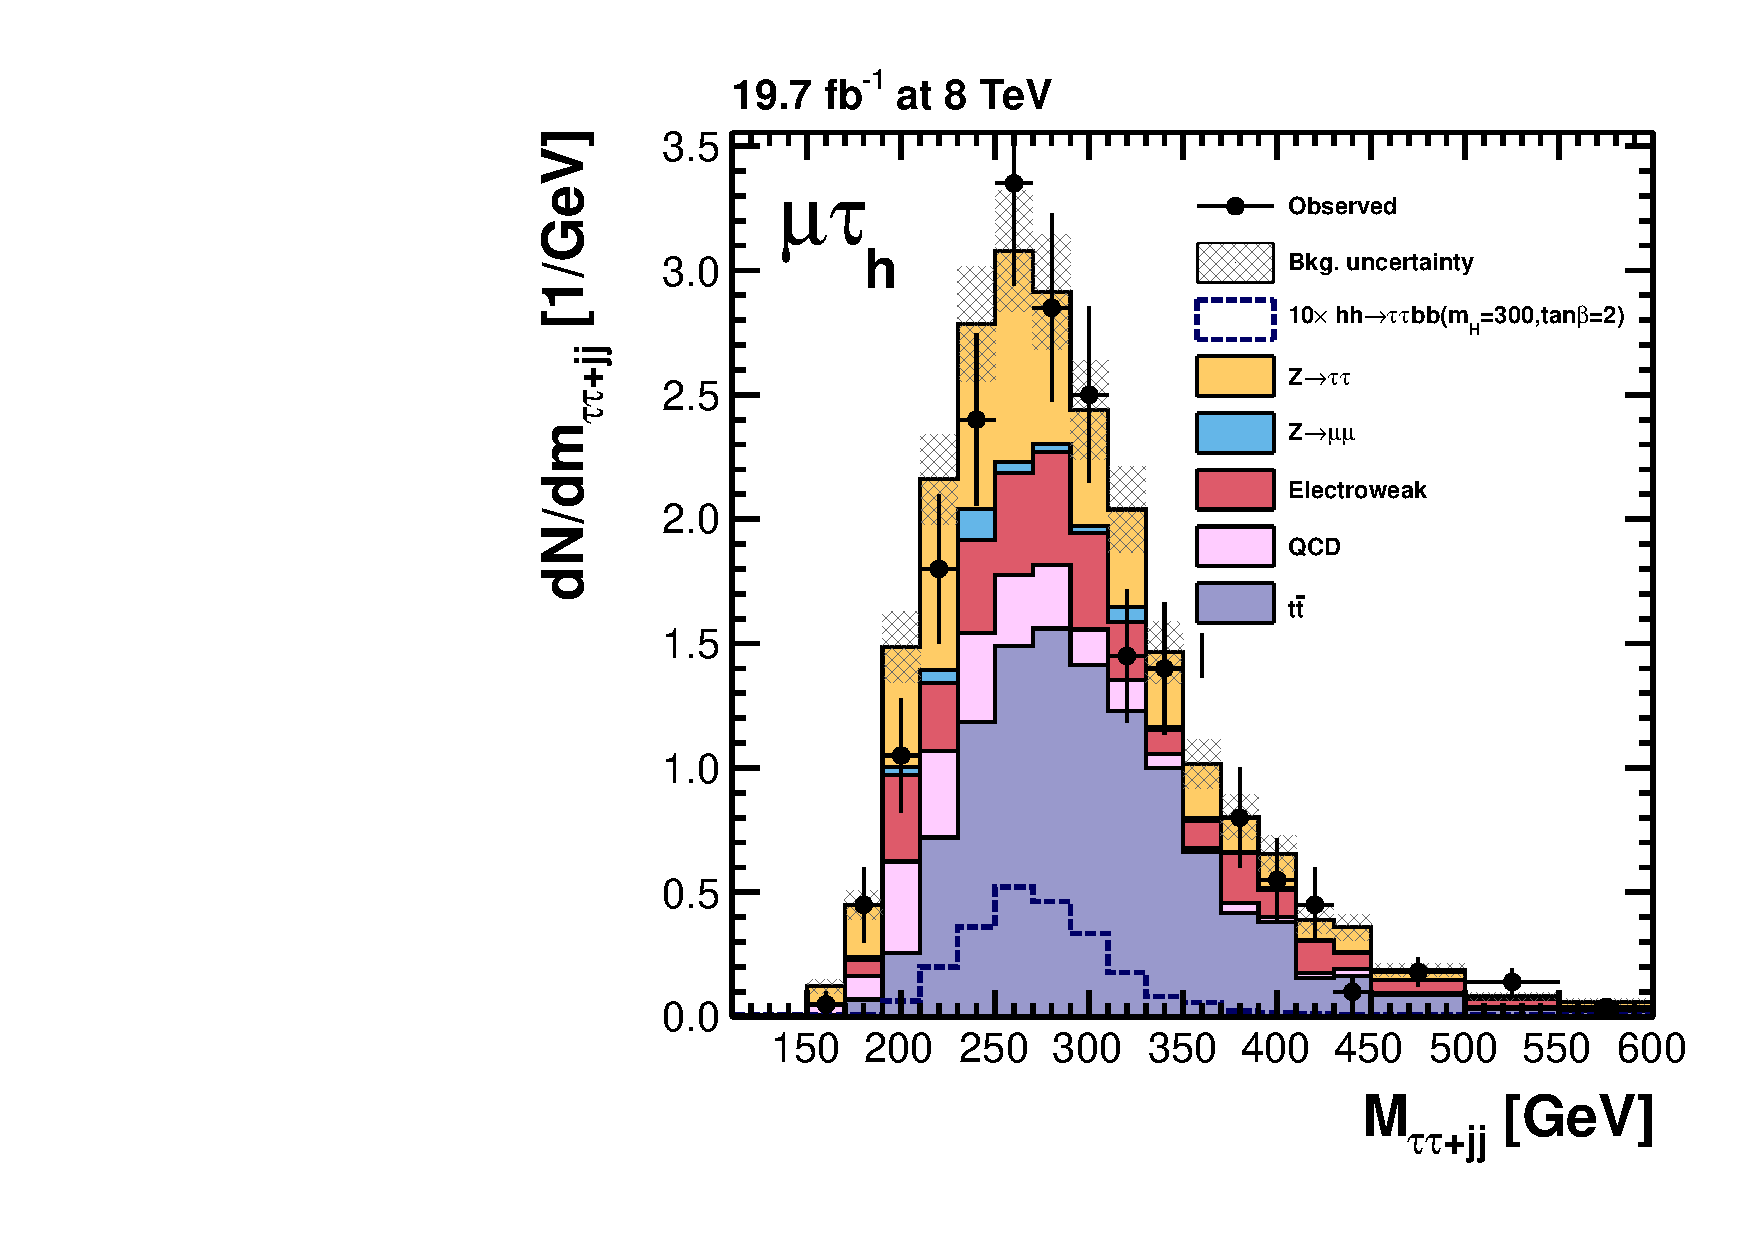
\includegraphics[width=0.5\textwidth]
      {plots/Hhh/mjj_tt_2jet1tagSFMassCuts_mt_2012.pdf}}
\subfloat[]{
    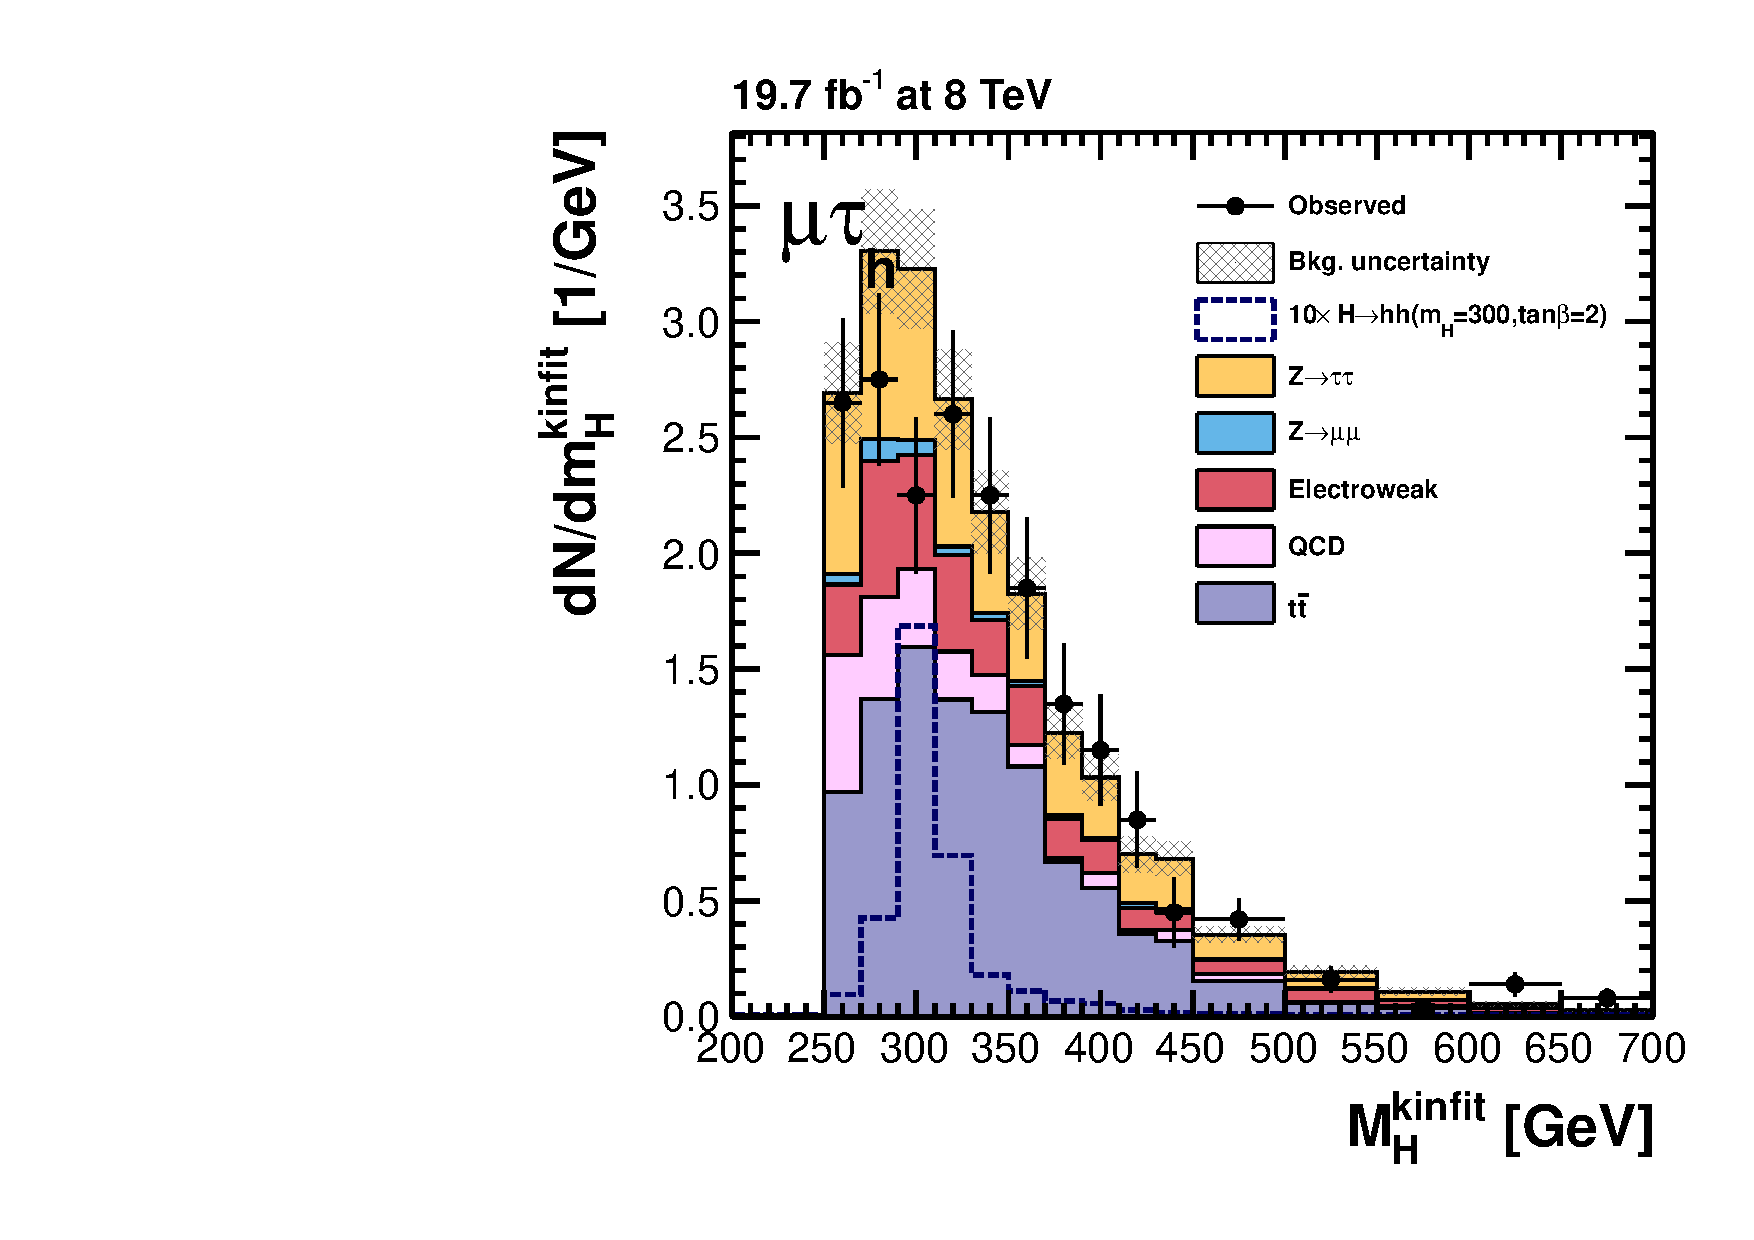
\includegraphics[width=0.5\textwidth]
      {plots/Hhh/m_H_hh_2jet1tagSFMassCuts_mt_2012.pdf}}

\end{center}
\caption{
Four body mass of the candidate \PH as reconstructed using a simple sum of the
individual components (left) or using a kinematic fit (right) as
described in the text. Shown for events in the 2jet--2tag category of the
$\mutau$ channel. The effect of the kinematic fit on the backgrounds is to force
a minimum at $2\times125=250~\GeV$, but otherwise the shapes are largely
unchanged.}
\label{fig:kinfitvsmttbb}
\end{figure} 

\section{Background methods}
\label{sec:Hhhbackgrounds}

Inclusively, the background composition is the same as discussed in the previous
chapters. The additional requirement that the events contain at least two jets
changes the composition slighly, with the largest effect being an increase in
$\ttbar$ background and a decrease in $\ZToTauTau$, $\WJets$ and QCD. The
variation with category is large, with 2jet--0tag events containing mostly
$\ZToTauTau$, $\WJets$ and QCD, and 2jet--2tag events containing almost entirely
$\ttbar$. In general the background methods follow those described in the
previous chapters, with the exception of adaptations necessary to deal with the
increased amount of $\ttbar$ and the generally lower statistics in the
categories after applying the mass cuts on $m_{\Pqb\Pqb}$ and $m_{\Pgt\Pgt}$.

\subsection{$\ZToTauTau$}

\subsection{$\ttbar$}

\begin{figure}
\begin{center}
\subfloat[]{
    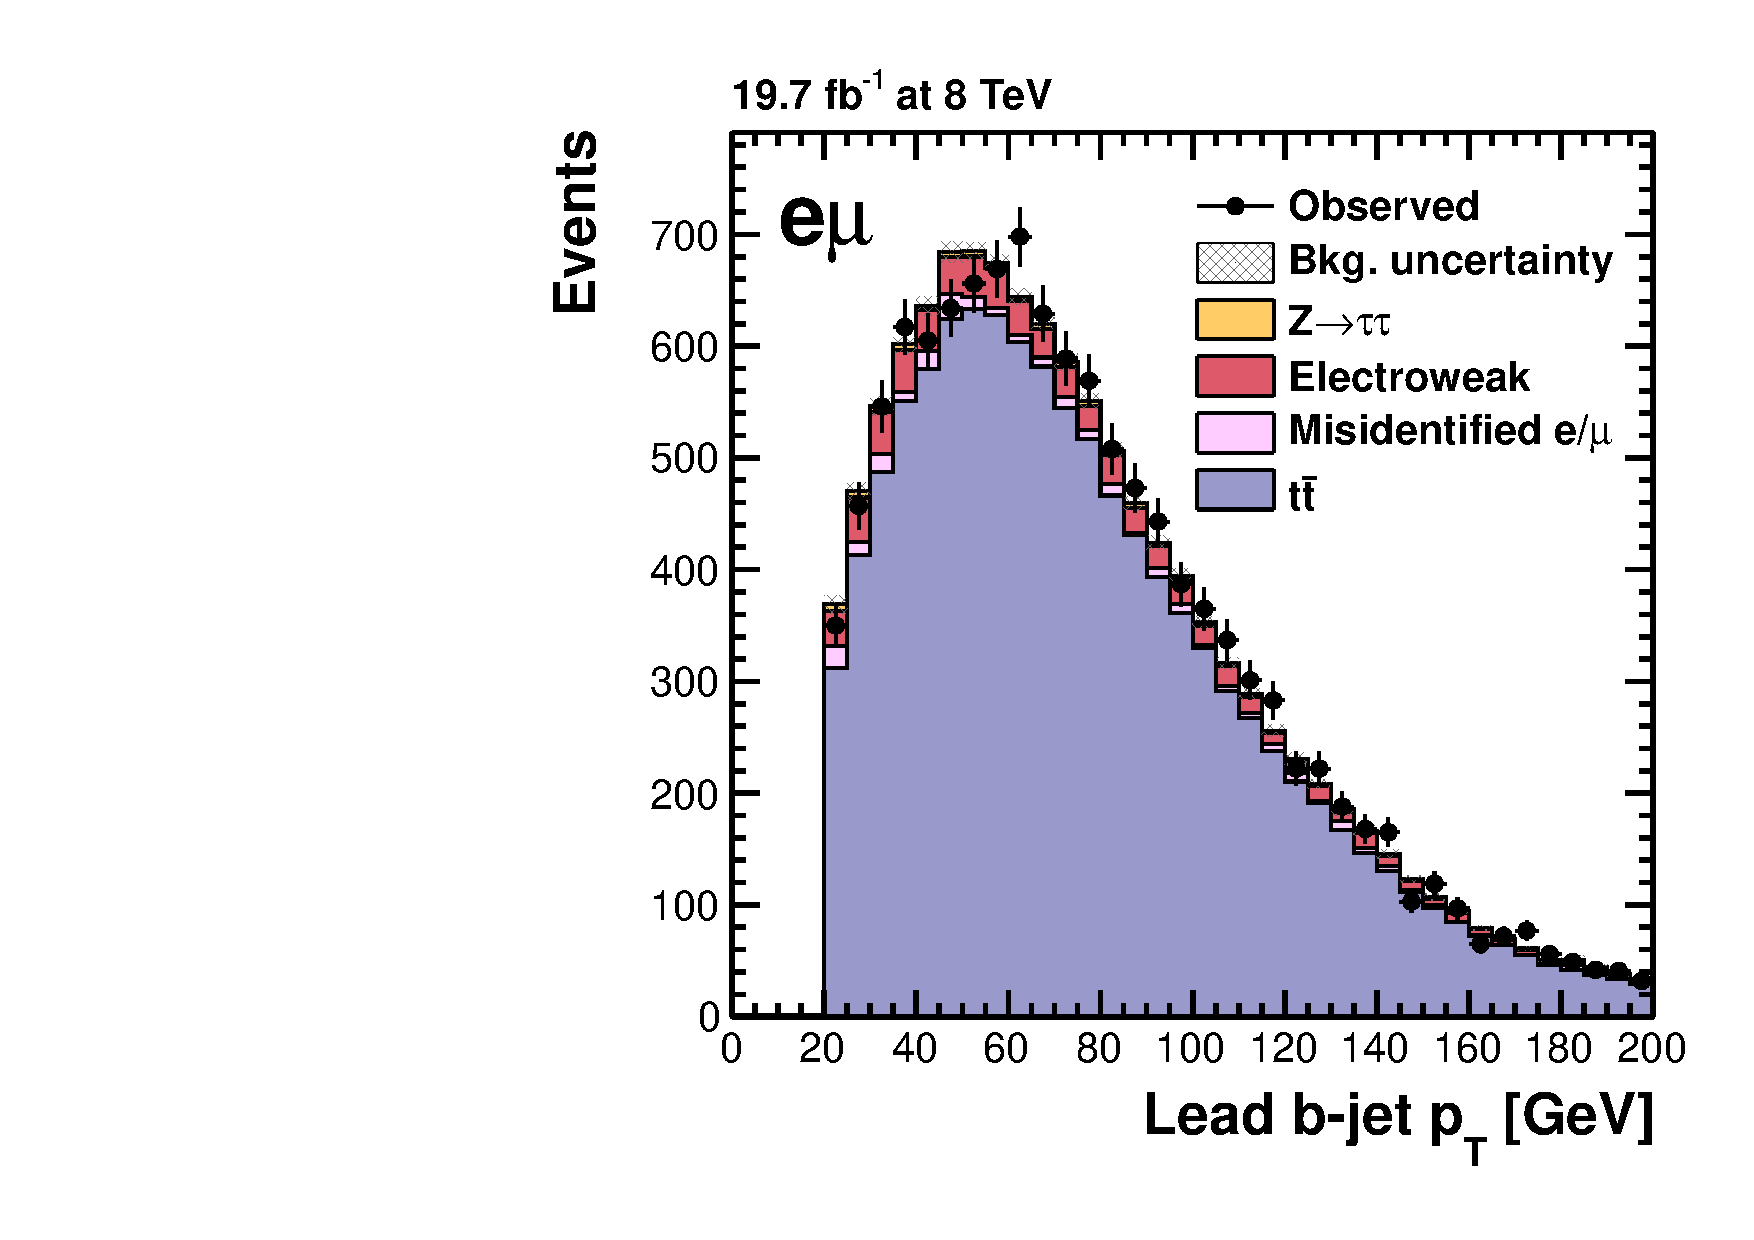
\includegraphics[width=0.5\textwidth]
      {plots/Hhh/TTBarControl/prebjetpt_1_2jetGT1tagSF_em_2012.pdf}}
\subfloat[]{
    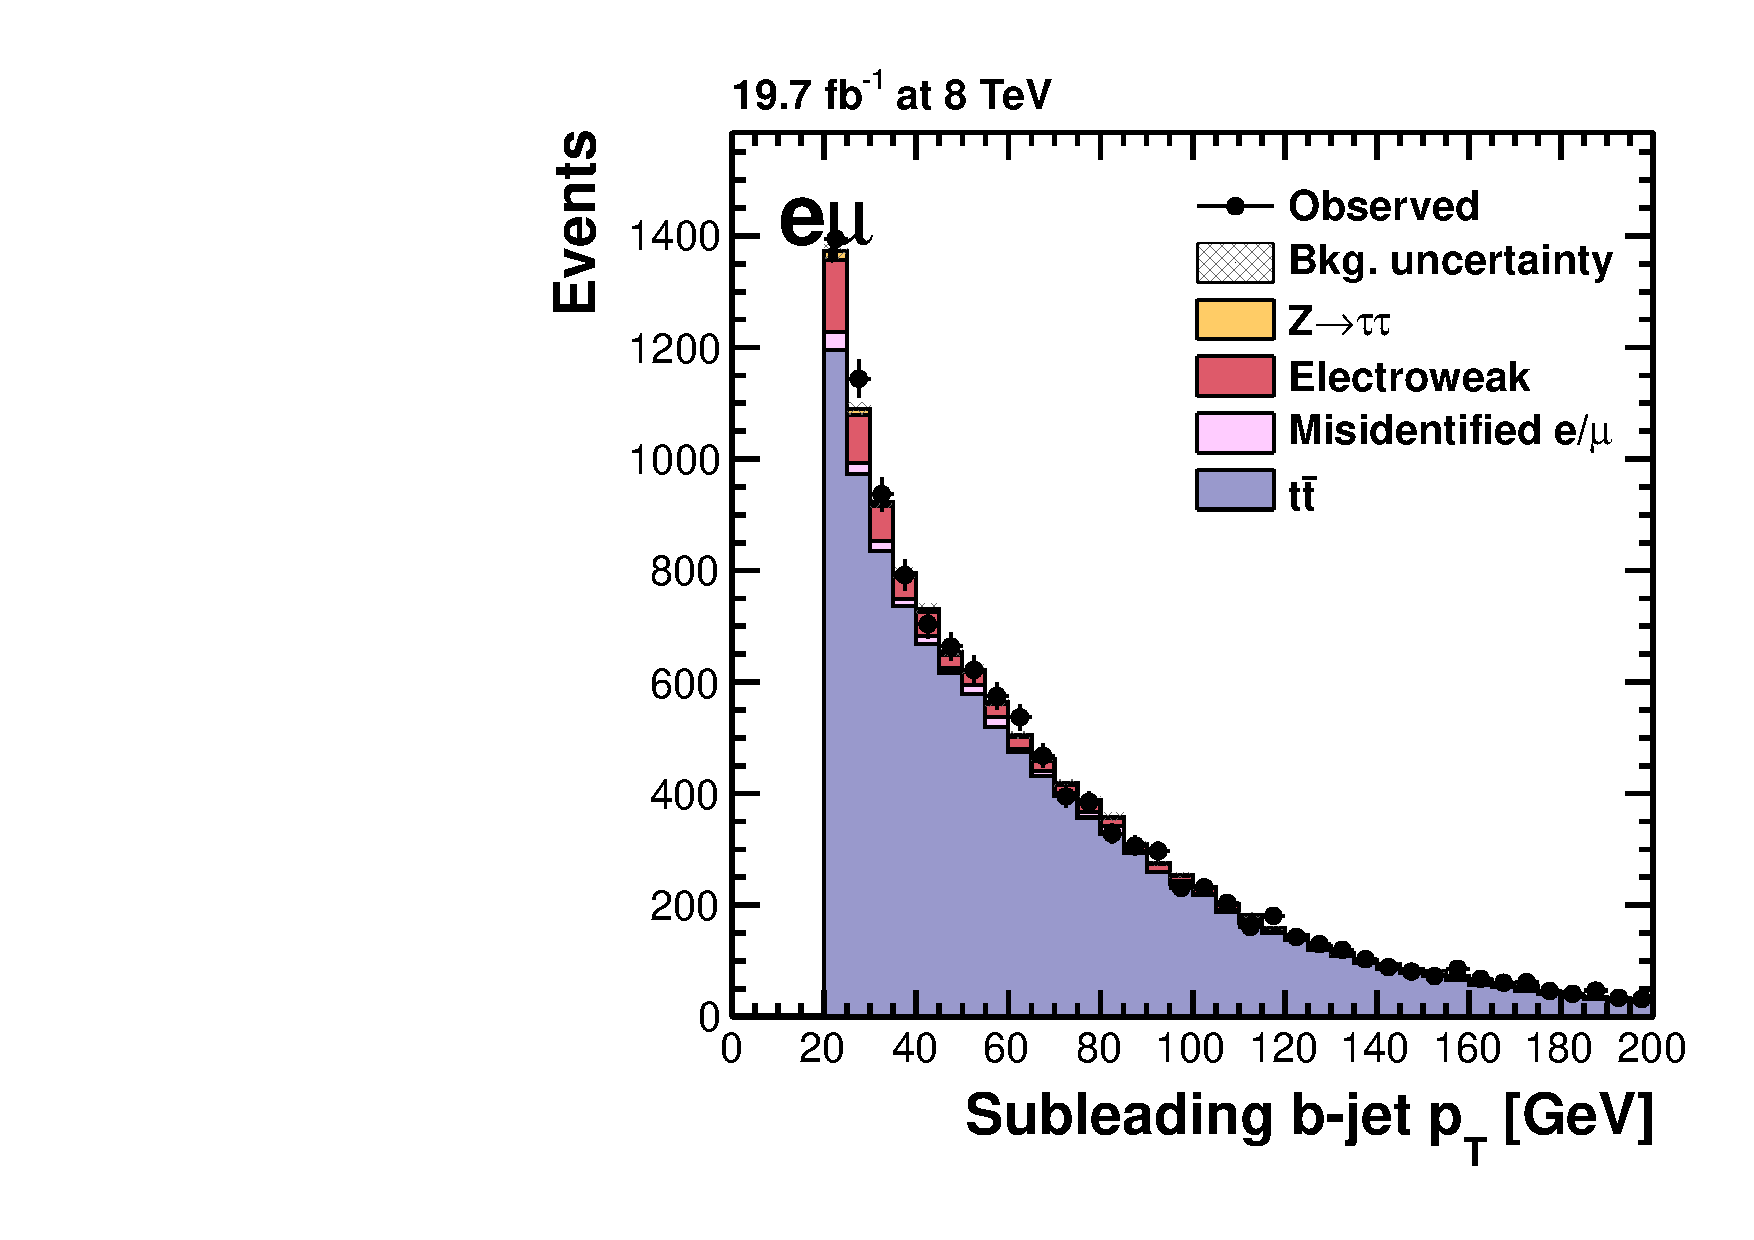
\includegraphics[width=0.5\textwidth]
      {plots/Hhh/TTBarControl/prebjetpt_2_2jetGT1tagSF_em_2012.pdf}}

\subfloat[]{
    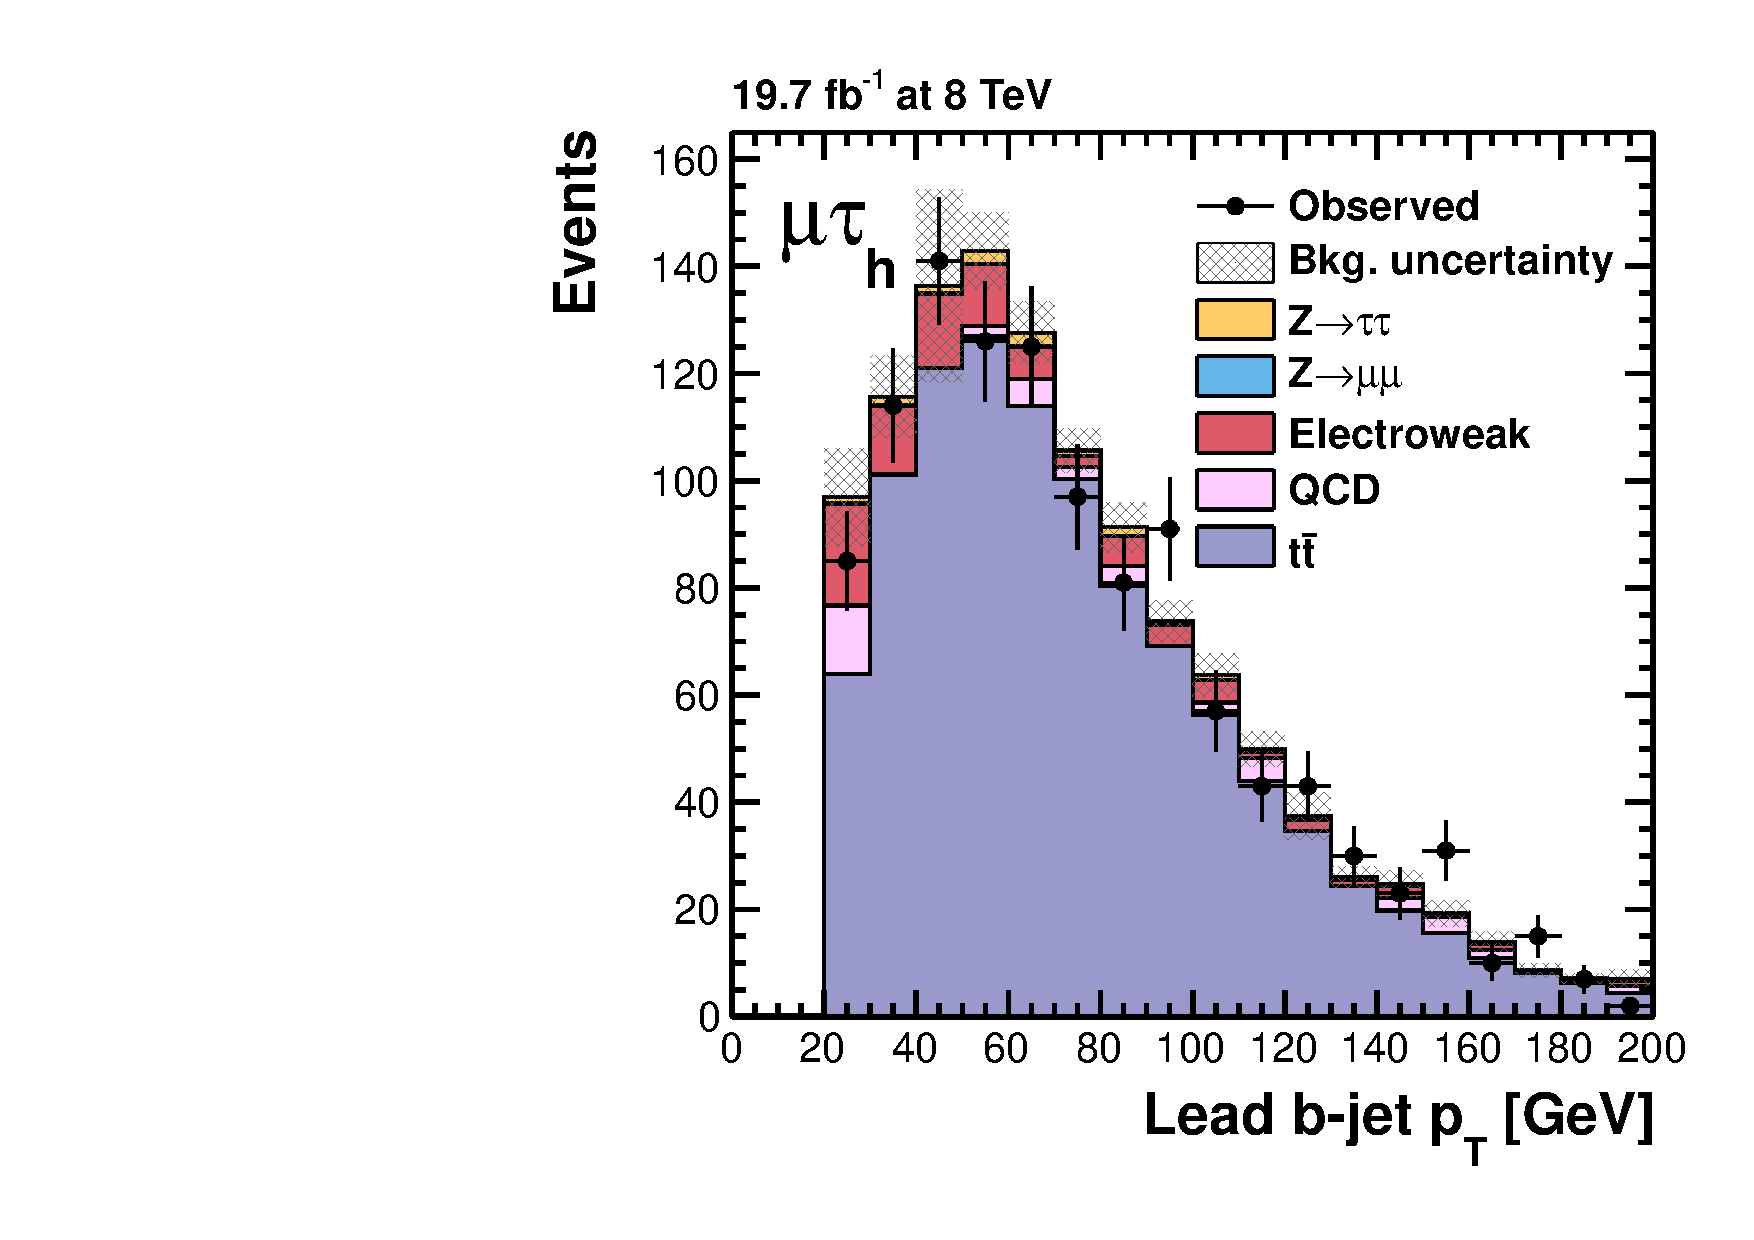
\includegraphics[width=0.5\textwidth]
      {plots/Hhh/TTBarControl/prebjetpt_1_2jet2tagSF_mt_2012.pdf}}
\subfloat[]{
    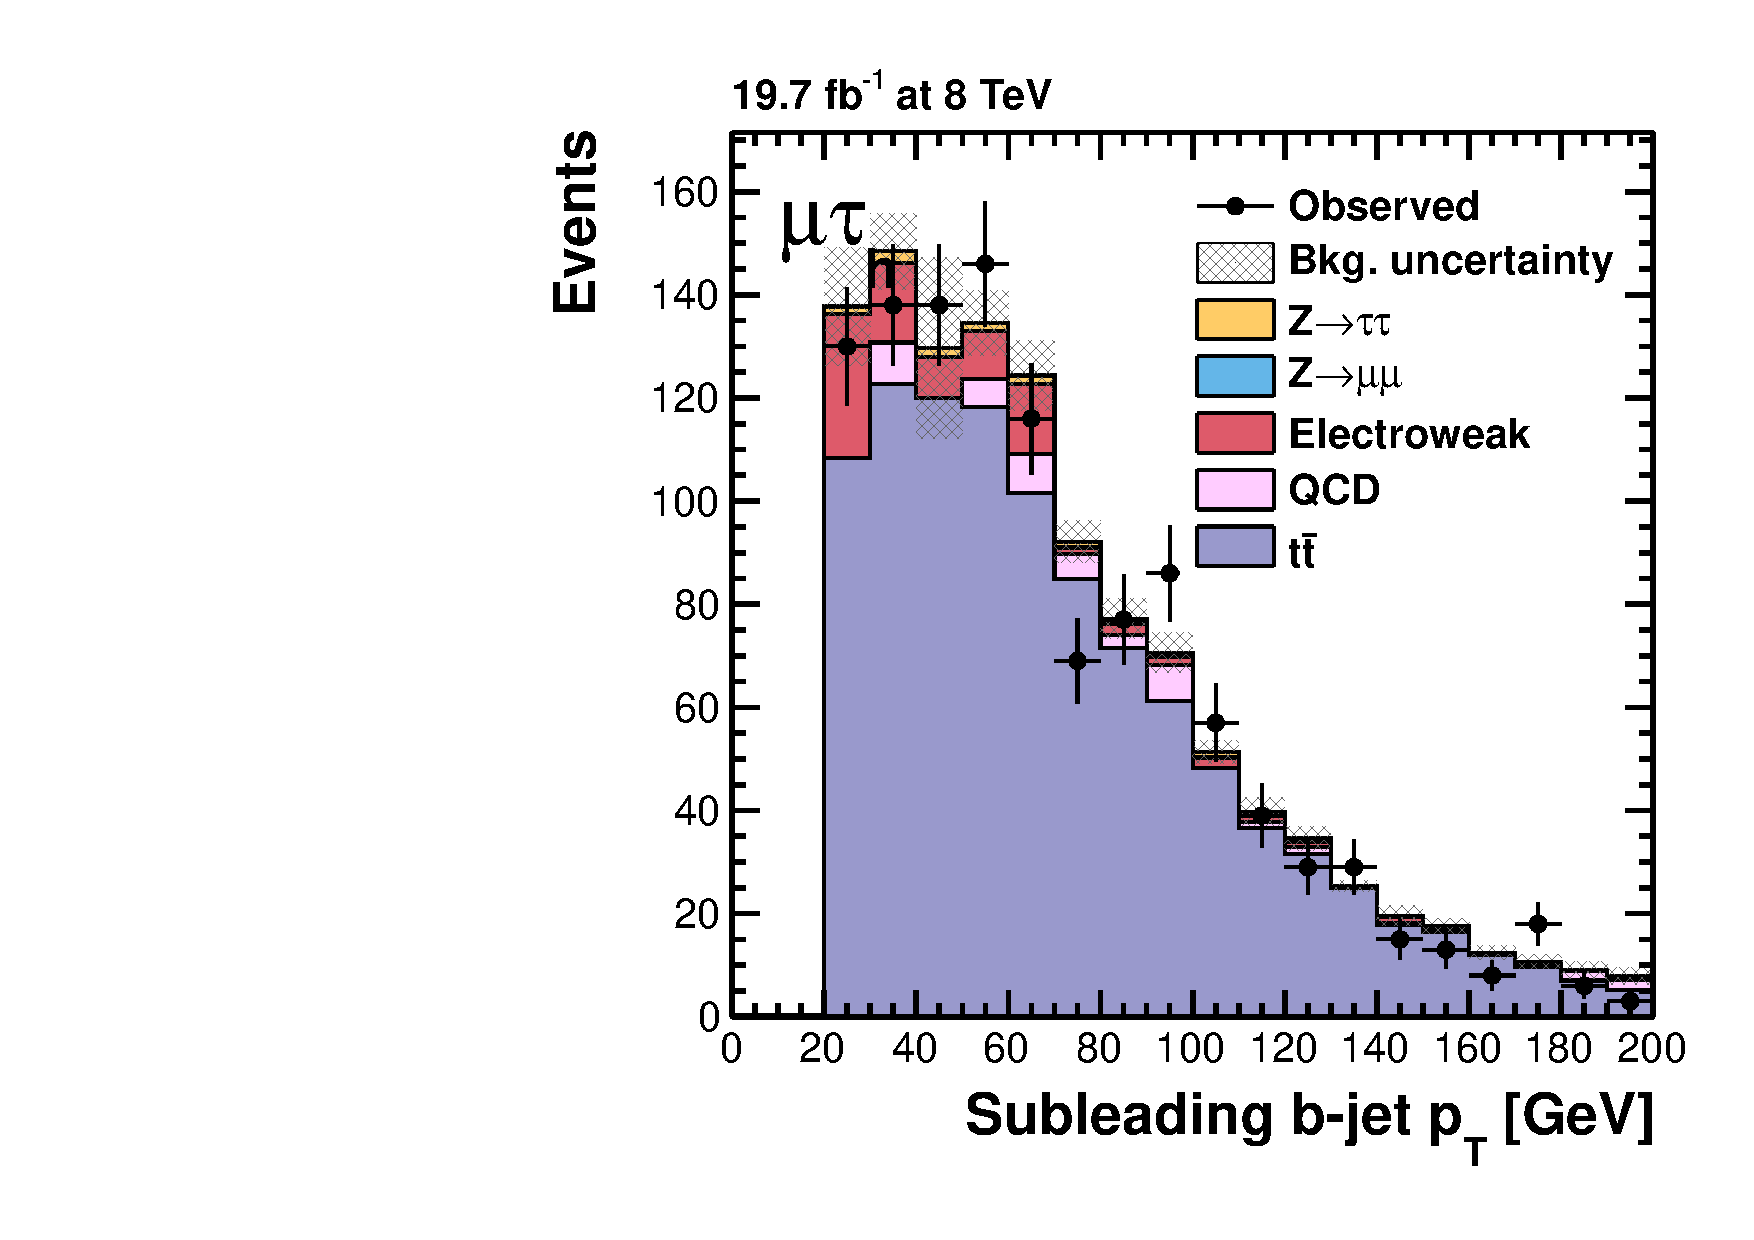
\includegraphics[width=0.5\textwidth]
      {plots/Hhh/TTBarControl/prebjetpt_2_2jet2tagSF_mt_2012.pdf}}
\end{center}
\caption{
Leading and subleading b-jet $\pt$ in the $\ttbar$ control regions for the
$\emu$ and $\mutau$ channels as defined in the text..}
\label{fig:ttbarcontrol}
\end{figure} 

\subsection{$\WJets$}

\subsection{QCD}

\subsection{$\PZ\to\ell\ell$, single top and diboson}

\section{Systematic uncertainties}
\label{sec:Hhhsystematics}

